\documentclass{article}
%% 1. CÀI ĐẶT CƠ BẢN & LỚP VĂN BẢN
\usepackage[utf8]{inputenc}
% \usepackage[T5]{fontenc} % Bỏ dòng này vì đã có T1 bên dưới, tránh xung đột
\usepackage[T1]{fontenc}
\usepackage[table,xcdraw]{xcolor}
\usepackage{tikz}
\usepackage{tcolorbox}

%% 2. BỐ CỤC TRANG & CANH LỀ (ĐÃ SỬA THEO YÊU CẦU)
\usepackage[a4paper, top=3.5cm, bottom=3cm, left=3.5cm, right=2cm]{geometry}
% Đã BỎ tùy chọn "twoside" để lề trang không bị lệch


%% 3. NGÔN NGỮ, FONT CHỮ & ĐỊNH DẠNG ĐOẠN VĂN (ĐÃ SỬA THEO YÊU CẦU)
\usepackage[vietnamese]{babel}
\usepackage{mathptmx} % Font Times New Roman
\usepackage{indentfirst}
% --- CÀI ĐẶT FONT, GIÃN DÒNG, THỤT LỀ MỚI ---
\renewcommand{\normalsize}{\fontsize{13}{15.6}\selectfont}
\linespread{1.5} % Giãn dòng 1.5
\setlength{\parindent}{1cm} % Thụt đầu dòng 1cm
\setlength{\parskip}{10pt} % Khoảng cách giữa các đoạn là 10pt
\setlength{\emergencystretch}{2em}


%% 4. TÙY CHỈNH CÁC CẤP ĐỀ MỤC (SECTION, SUBSECTION,...)
\usepackage{titlesec}
\setcounter{secnumdepth}{4}

% Định dạng cho các chương CÓ ĐÁNH SỐ 
\titleformat{\section}[block]
  {\fontsize{16pt}{0pt}\selectfont \bfseries \centering}
  {CHƯƠNG \thesection:}
  {0.5em}
  {}
\titlespacing*{\section}{0pt}{0pt}{15pt}

% Định dạng cho các chương KHÔNG ĐÁNH SỐ
\titleformat{name=\section,numberless}[display]
  {\fontsize{16pt}{0pt}\selectfont \bfseries \centering}
  {}
  {0em}
  {}

% Định dạng cho các mục con
\titleformat*{\subsection}{\fontsize{14pt}{0pt}\selectfont \bfseries}
\titlespacing*{\subsection}{0pt}{3pt}{0pt}

\titleformat*{\subsubsection}{\fontsize{13pt}{0pt}\selectfont \bfseries \itshape}
\titlespacing*{\subsubsection}{0pt}{6pt}{0pt}

\titleformat*{\paragraph}{\fontsize{13pt}{0pt}\selectfont \itshape}
\titlespacing*{\paragraph}{0pt}{0pt}{0pt}

\titleformat{\paragraph}
  {\normalfont\fontsize{13pt}{0pt}\selectfont\itshape}
  {\theparagraph}
  {1em}
  {}
\titlespacing*{\paragraph}{0pt}{0.5ex plus 0.5ex minus .2ex}{0.5ex plus .2ex}


%% 5. HÌNH ẢNH, BẢNG BIỂU & CHÚ THÍCH (CAPTION)
\usepackage[nottoc]{tocbibind}
\usepackage{tocloft}
\setlength{\cftbeforesecskip}{6pt}
\setlength{\cftbeforesubsecskip}{2pt}
\setlength{\cftbeforesubsubsecskip}{1pt}

% Căn giữa các tiêu đề danh mục tương tự tiêu đề section gốc
\renewcommand{\cfttoctitlefont}{\hspace*{\fill}\fontsize{16pt}{0pt}\selectfont\bfseries}
\renewcommand{\cftaftertoctitle}{\hspace*{\fill}}
\renewcommand{\cftloftitlefont}{\hspace*{\fill}\fontsize{16pt}{0pt}\selectfont\bfseries}
\renewcommand{\cftafterloftitle}{\hspace*{\fill}}
\renewcommand{\cftlottitlefont}{\hspace*{\fill}\fontsize{16pt}{0pt}\selectfont\bfseries}
\renewcommand{\cftafterlottitle}{\hspace*{\fill}}
\usepackage{graphicx}
\usepackage{float}
\usepackage{longtable}
\usepackage{tabularx}
\usepackage{multirow}
\usepackage[font=normal]{caption}
\usepackage{array}

\renewcommand{\figurename}{\fontsize{12pt}{0pt}\selectfont Hình}
\captionsetup[figure]{labelsep=space}

\renewcommand{\tablename}{\fontsize{12pt}{0pt}\selectfont Bảng}
\captionsetup[table]{labelsep=space}

\newcolumntype{s}{>{\hsize=.3\hsize}X}
\newcolumntype{y}{>{\hsize=.4\hsize}X}
\newcolumntype{d}{>{\hsize=.1\hsize}X}
\newcolumntype{a}{>{\hsize=1.1\hsize}X}
\newcolumntype{g}{>{\hsize=5\hsize}X}
\newcolumntype{P}[1]{>{\raggedright\arraybackslash}p{#1}}
% --- SỬA LỖI TẠI ĐÂY ---
% \renewcommand{\tabularxcolumn}[1]{>{\small}m{#1}} % Dòng lệnh cũ gây lỗi thu nhỏ chữ
\renewcommand{\tabularxcolumn}[1]{>{\raggedright\arraybackslash}m{#1}} % Lệnh mới: Bỏ \small, thêm căn lề trái cho đẹp
% -----------------------


% Cho phép xếp nhiều hình/bảng trên một trang để giảm khoảng trắng
\renewcommand{\topfraction}{0.85}
\renewcommand{\bottomfraction}{0.7}
\renewcommand{\textfraction}{0.1}
\renewcommand{\floatpagefraction}{0.75}
\setcounter{topnumber}{3}
\setcounter{bottomnumber}{2}
\setcounter{totalnumber}{5}


%% 6. KHỐI LỆNH (CODE LISTINGS) 
\usepackage{listings}
% Gói xcolor đã được nạp ở mục 5, không cần nạp lại

\lstdefinestyle{customcode}{
    basicstyle=\small\ttfamily,
    breaklines=true,
    numbers=left,
    numberstyle=\tiny\color{gray},
    keywordstyle=\color{blue!80!black}\bfseries,
    commentstyle=\color{green!50!black}\itshape,
    stringstyle=\color{red!70!black},
    showstringspaces=false,
    tabsize=2,
    captionpos=b,
    frame=single,
    rulecolor=\color{gray!40},
    xleftmargin=1.5em,
    framexleftmargin=1em,
    aboveskip=1.5em,
    belowskip=1.5em
}
\renewcommand{\lstlistingname}{Khối lệnh}


%% 7. TOÁN HỌC & CÁC MÔI TRƯỜNG ĐỊNH LÝ
\newtheorem{theorem}{Định lý}[section]
\newtheorem{defn}[theorem]{Định nghĩa}
\newtheorem{corollary}[theorem]{Hệ quả}
\newtheorem{lemma}[theorem]{Bổ đề}


%% 8. TÀI LIỆU THAM KHẢO
\usepackage[natbibapa]{apacite} 
\bibliographystyle{apacite}
\makeatletter
\def\APAC@apcfile{english.apc}
\makeatother

%% 9. CÁC GÓI BỔ SUNG KHÁC
\usepackage{wrapfig}
% Gói tikz đã được nạp ở mục 1, không cần nạp lại
\usetikzlibrary{calc,backgrounds,fit}
\usepackage{soul}
\usepackage{colortbl}
\usepackage{forloop}
\usepackage{enumitem}

\definecolor{LightCyan}{rgb}{0.88,1,1}
\newcounter{loopcntr}
\newcommand{\rpt}[2][1]{\forloop{loopcntr}{0}{\value{loopcntr}<#1}{#2}}
\setitemize{itemsep=0pt,leftmargin=1.25cm,topsep = 3pt}


%% 10. ĐÁNH SỐ TỰ ĐỘNG & LIÊN KẾT 
\usepackage{chngcntr}
\usepackage[unicode, plainpages=false, pdfpagelabels=true, hidelinks]{hyperref}

% Cấu hình bộ đếm cho các môi trường
\counterwithin{figure}{section}
\counterwithin{table}{section}
\counterwithin{equation}{section}
% Các counter khác đã được article class và titlesec xử lý, không cần thêm


%% 11. ĐỊNH NGHĨA LẠI TÊN CÁC THÀNH PHẦN CỦA TÀI LIỆU
\AtBeginDocument{%
  \renewcommand{\contentsname}{MỤC LỤC}
  \renewcommand{\listfigurename}{DANH MỤC HÌNH VẼ}
  \renewcommand{\listtablename}{DANH MỤC BẢNG BIỂU}
  \renewcommand{\refname}{TÀI LIỆU THAM KHẢO}
  \normalsize % Áp dụng cỡ chữ mặc định cho toàn bộ tài liệu
}


%% 12. CÁC BIẾN TOÀN CỤC SỬ DỤNG TRONG BÁO CÁO
\newcommand{\khoa}{CÔNG NGHỆ THÔNG TIN}
\newcommand{\mon}{ĐỒ ÁN TỐT NGHIỆP}
\newcommand{\chuyennganh}{MẠNG MÁY TÍNH VÀ TRUYỀN THÔNG DỮ LIỆU}
\newcommand{\de}{XÂY DỰNG NỀN TẢNG GÂY QUỸ CỘNG ĐỒNG CHO CÁC DỰ ÁN XÃ HỘI VÀ KHỞI NGHIỆP}
\newcommand{\gvhd}{ThS. DƯƠNG HỮU PHƯỚC}
\newcommand{\svmot}{TRẦN HỮU NHÂN - 52300235}
\newcommand{\svhai}{NGUYỄN NHẬT HÀO - 52300198}
\newcommand{\lop}{23050401}
\newcommand{\khoahoc}{27}
\newcommand{\nam}{2026}

\newcommand{\loaibaocao}{TÀI LIỆU ĐẶC TẢ ERD}
\newcommand{\mocbaocao}{28/10/2026}
 % Dùng chung preamble với báo cáo chính

\begin{document}

	% --- PHẦN BÌA (KHÔNG ĐÁNH SỐ) ---
	\hypersetup{pageanchor=false}
	\pagenumbering{gobble}

	\pagenumbering{gobble}
\begin{center}
	\fontsize{14pt}{0pt}\selectfont TỔNG LIÊN ĐOÀN LAO ĐỘNG VIỆT NAM \\
	\fontsize{14pt}{0pt}\selectfont \textbf{TRƯỜNG ĐẠI HỌC TÔN ĐỨC THẮNG} \\
	\fontsize{14pt}{0pt}\selectfont \textbf{KHOA \khoa} \\\vspace*{6 pt}		
\includegraphics[width=0.3\linewidth]{image/logo-tdtu.jpg}\\\vspace*{0.3cm}

	\fontsize{14pt}{0pt}\selectfont \textbf{\svmot}\\\vspace{6pt}
    \fontsize{14pt}{0pt}\selectfont \textbf{\svhai}\\\vspace{11pt}
    \vspace*{2.5cm}
	\fontsize{24pt}{0pt}\selectfont 
    \textbf{\de}\\\vspace*{2cm}
    
	\fontsize{20pt}{0pt}\selectfont \textbf{\loaibaocao}\\\vspace*{10pt}
	\fontsize{18pt}{0pt}\selectfont \textbf{\mon}\\\vspace*{6pt}
        \fontsize{18pt}{0pt}\selectfont \textbf{\chuyennganh}\\\vspace*{2.5cm}
 
	\fontsize{14pt}{0pt}\selectfont \textbf{THÀNH PHỐ HỒ CHÍ MINH, \nam} \\
  
\end{center}
\newpage
      % Trang bìa 1
	\begin{center}
	\fontsize{14pt}{0pt}\selectfont TỔNG LIÊN ĐOÀN LAO ĐỘNG VIỆT NAM \\
	\fontsize{14pt}{0pt}\selectfont \textbf{TRƯỜNG ĐẠI HỌC TÔN ĐỨC THẮNG} \\
	\fontsize{14pt}{0pt}\selectfont \textbf{KHOA \khoa} \\\vspace*{6pt}	
    
\includegraphics[width=0.3\linewidth]{image/logo-tdtu.jpg}\\\vspace*{0.5cm}
 
	\fontsize{14pt}{0pt}\selectfont \textbf{\svmot}\\\vspace{6pt}
    \fontsize{14pt}{0pt}\selectfont \textbf{\svhai}\\\vspace{11pt}

    \vspace*{1cm}

	\fontsize{24pt}{0pt}\selectfont \textbf{\de}\\\vspace*{1cm}

	\fontsize{20pt}{0pt}\selectfont \textbf{\loaibaocao}\\\vspace*{10pt}
	\fontsize{18pt}{0pt}\selectfont \textbf{\mon}\\\vspace*{6pt}
        \fontsize{18pt}{0pt}\selectfont \textbf{\chuyennganh}\\\vspace*{0.8cm}
        
        \fontsize{14pt}{0pt}\selectfont Người hướng dẫn\\\vspace{6pt}
	\fontsize{14pt}{0pt}\selectfont \textbf{\gvhd} \\\vspace*{0.8cm}
 
	\fontsize{14pt}{0pt}\selectfont \textbf{THÀNH PHỐ HỒ CHÍ MINH, \nam} \\
  
\end{center}	
\newpage
   % Trang bìa 2

	% --- PHẦN ĐẦU CỦA TÀI LIỆU ---
	\cleardoublepage
	\hypersetup{pageanchor=true}
	\pagenumbering{roman}
	\setcounter{page}{3}

	\section*{\fontsize{18pt}{18pt}\selectfont\MakeUppercase{\de}\\TÓM TẮT TÀI LIỆU ĐẶC TẢ ERD}

Tài liệu đặc tả mô hình dữ liệu của nền tảng gây quỹ cộng đồng Góp Mầm (phiên bản 1.1, cập nhật ngày 27/10/2026). Cơ sở dữ liệu chạy trên MySQL 8 với engine InnoDB; schema chỉ thay đổi qua migration TypeORM có thứ tự và có rollback.

Hệ thống gồm 24 thực thể chia thành sáu nhóm: tài khoản, chiến dịch và tiến độ, giao dịch, cộng đồng, kiểm duyệt và rủi ro, AI và hệ thống. Giữa các thực thể có 37 mối quan hệ có khóa ngoại (36 quan hệ 1-N, 1 quan hệ 1-1) và 5 tham chiếu logic không đặt khóa ngoại. Mọi khóa chính là UUID dạng \texttt{CHAR(36)}, trừ hai ngoại lệ có giải thích.

Thiết kế dữ liệu ưu tiên tính toàn vẹn của giao dịch tài chính: khóa idempotency và các ràng buộc UNIQUE chống ghi nhận trùng, số tiền đã huy động chỉ cộng từ khoản ủng hộ đã xác minh, thao tác hoàn tiền yêu cầu mã OTP, dữ liệu quan trọng dùng xóa mềm và mọi thay đổi được ghi nhật ký kiểm toán. Việc giải ngân được minh bạch bằng chứng từ chi tiêu, nhắc mốc quá hạn và lịch sử thay đổi kế hoạch công khai.

Tài liệu gồm năm chương: tổng quan hệ thống và sơ đồ ERD; đặc tả từng thực thể; các mối quan hệ; quy trình nghiệp vụ theo dữ liệu; các điểm lưu ý đặc biệt và tổng kết.

\textbf{Từ khóa:} ERD, cơ sở dữ liệu, MySQL, InnoDB, khóa ngoại, migration, crowdfunding.

\newpage


	\tableofcontents
	\newpage

	\listoffigures
	\newpage

	\listoftables
	\newpage

	\newpage
\section*{DANH MỤC CÁC TỪ VIẾT TẮT}
\addcontentsline{toc}{section}{DANH MỤC CÁC TỪ VIẾT TẮT}

{
\renewcommand{\arraystretch}{1.3}
\begin{longtable}{ >{\centering\arraybackslash}p{3cm} p{9cm} }
    \textbf{Viết tắt} & \textbf{Tiếng Anh} \\

    AI & Artificial Intelligence \\
    API & Application Programming Interface \\
    CSDL & Cơ sở dữ liệu \\
    DBML & Database Markup Language \\
    ENUM & Enumeration \\
    ERD & Entity Relationship Diagram \\
    FK & Foreign Key \\
    HMAC & Hash-based Message Authentication Code \\
    IP & Internet Protocol \\
    JWT & JSON Web Token \\
    NGO & Non-Governmental Organization \\
    ORM & Object-Relational Mapping \\
    OTP & One-Time Password \\
    PK & Primary Key \\
    SHA & Secure Hash Algorithm \\
    UUID & Universally Unique Identifier \\
\end{longtable}
}


	% --- PHẦN THÂN CỦA TÀI LIỆU ---
	\newpage
	\pagenumbering{arabic}

	\section{TỔNG QUAN HỆ THỐNG}\label{sec:chuong1}

Hệ thống gây quỹ cộng đồng Góp Mầm được thiết kế để quản lý toàn bộ quy trình từ đăng ký tài khoản, tạo và kiểm duyệt chiến dịch, ủng hộ trực tuyến kèm mức quà, cập nhật tiến độ giải ngân có chứng từ, hoàn tiền, đến tương tác cộng đồng, kiểm duyệt vi phạm, phát hiện gian lận bằng AI, thông báo, xác minh tổ chức thụ hưởng và xác minh bổ sung bằng mã OTP cho thao tác nhạy cảm. Hệ thống gồm 24 thực thể với 37 mối quan hệ có khóa ngoại và 5 tham chiếu logic.

Hệ quản trị cơ sở dữ liệu: MySQL 8, engine InnoDB. Schema chỉ thay đổi qua migration TypeORM có thứ tự và có rollback (khớp tới migration 1790000000012).

Các thực thể được chia thành sáu nhóm nghiệp vụ như Bảng~\ref{tab:nhom_thuc_the}.

\begin{table}[htbp]
    \centering
    \small
    \caption{Các nhóm thực thể}
    \label{tab:nhom_thuc_the}
    \begin{tabularx}{\textwidth}{|P{3.6cm}|X|}
        \hline
        \textbf{Nhóm} & \textbf{Thực thể} \\
        \hline
        Tài khoản & USERS, EMAIL\_\allowbreak{}VERIFICATION\_\allowbreak{}TOKENS, PASSWORD\_\allowbreak{}RESET\_\allowbreak{}TOKENS, REVOKED\_\allowbreak{}TOKENS, STEP\_\allowbreak{}UP\_\allowbreak{}CODES \\
        \hline
        Chiến dịch và tiến độ & CAMPAIGNS, ORGANIZATIONS, CATEGORIES, CAMPAIGN\_\allowbreak{}VIEW\_\allowbreak{}DAILY, MILESTONES, MILESTONE\_\allowbreak{}UPDATES, MILESTONE\_\allowbreak{}UPDATE\_\allowbreak{}ATTACHMENTS, MILESTONE\_\allowbreak{}REVISIONS, REWARD\_\allowbreak{}TIERS, MEDIA\_\allowbreak{}FILES \\
        \hline
        Giao dịch & DONATIONS, REFUND\_\allowbreak{}REQUESTS \\
        \hline
        Cộng đồng & CAMPAIGN\_\allowbreak{}COMMENTS, CAMPAIGN\_\allowbreak{}FOLLOWS \\
        \hline
        Kiểm duyệt và rủi ro & REPORTS, RISK\_\allowbreak{}ALERTS \\
        \hline
        AI và hệ thống & BEHAVIOR\_\allowbreak{}EVENTS, NOTIFICATIONS, AUDIT\_\allowbreak{}LOGS \\
        \hline
    \end{tabularx}
\end{table}

\subsection{Sơ đồ ERD}

Sơ đồ dưới đây thể hiện các thực thể và quan hệ có khóa ngoại. Hình ERD vật lý đầy đủ cột được vẽ tự động (Graphviz) từ file DBML docs/database/schema.dbml.

\begin{figure}[htbp]
    \centering
    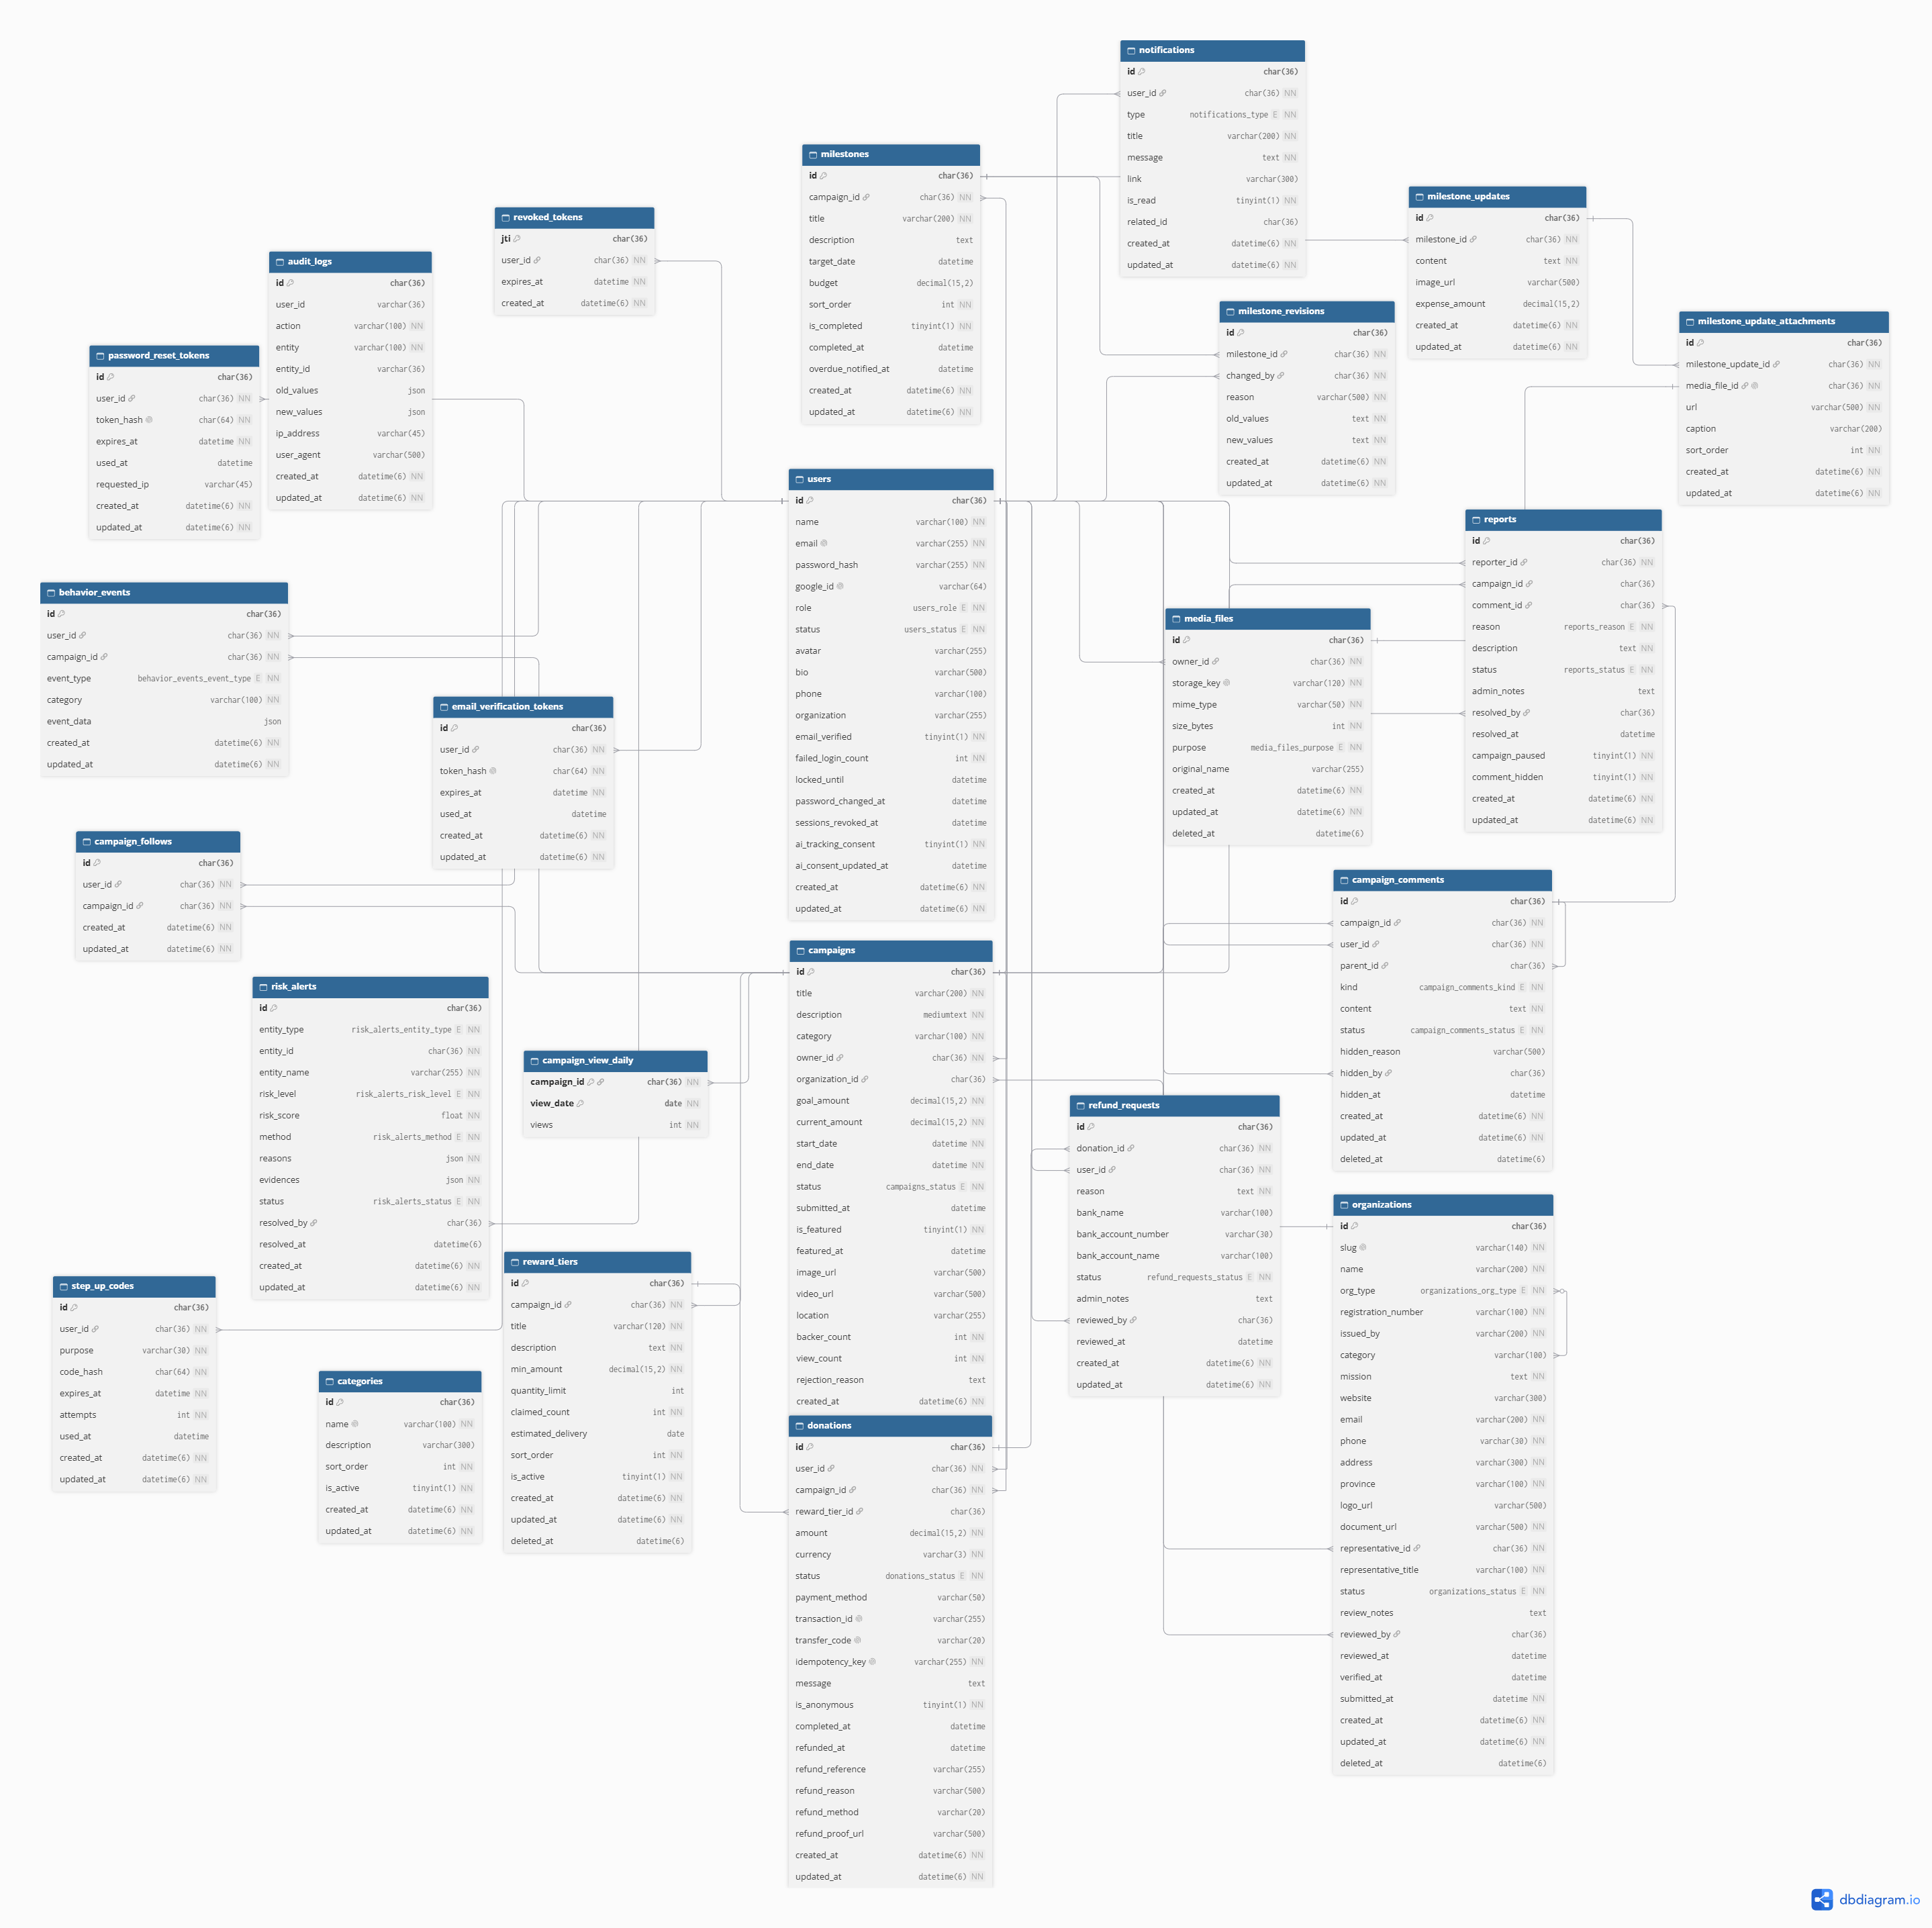
\includegraphics[width=\textwidth,height=0.72\textheight,keepaspectratio]{image/ERD_GopMam.png}
    \caption{Sơ đồ ERD vật lý hệ thống Góp Mầm (24 bảng)}
    \label{fig:erd_vat_ly}
\end{figure}

\subsection{Mô hình quan hệ}

Mô hình quan hệ (ký hiệu Chen) vẽ các thực thể bằng hình chữ nhật và quan hệ bằng hình thoi, tên quan hệ lấy theo các mục ở Chương 3. Sơ đồ lõi của hệ thống được vẽ ở cuối chương này.

\begin{figure}[htbp]
    \centering
    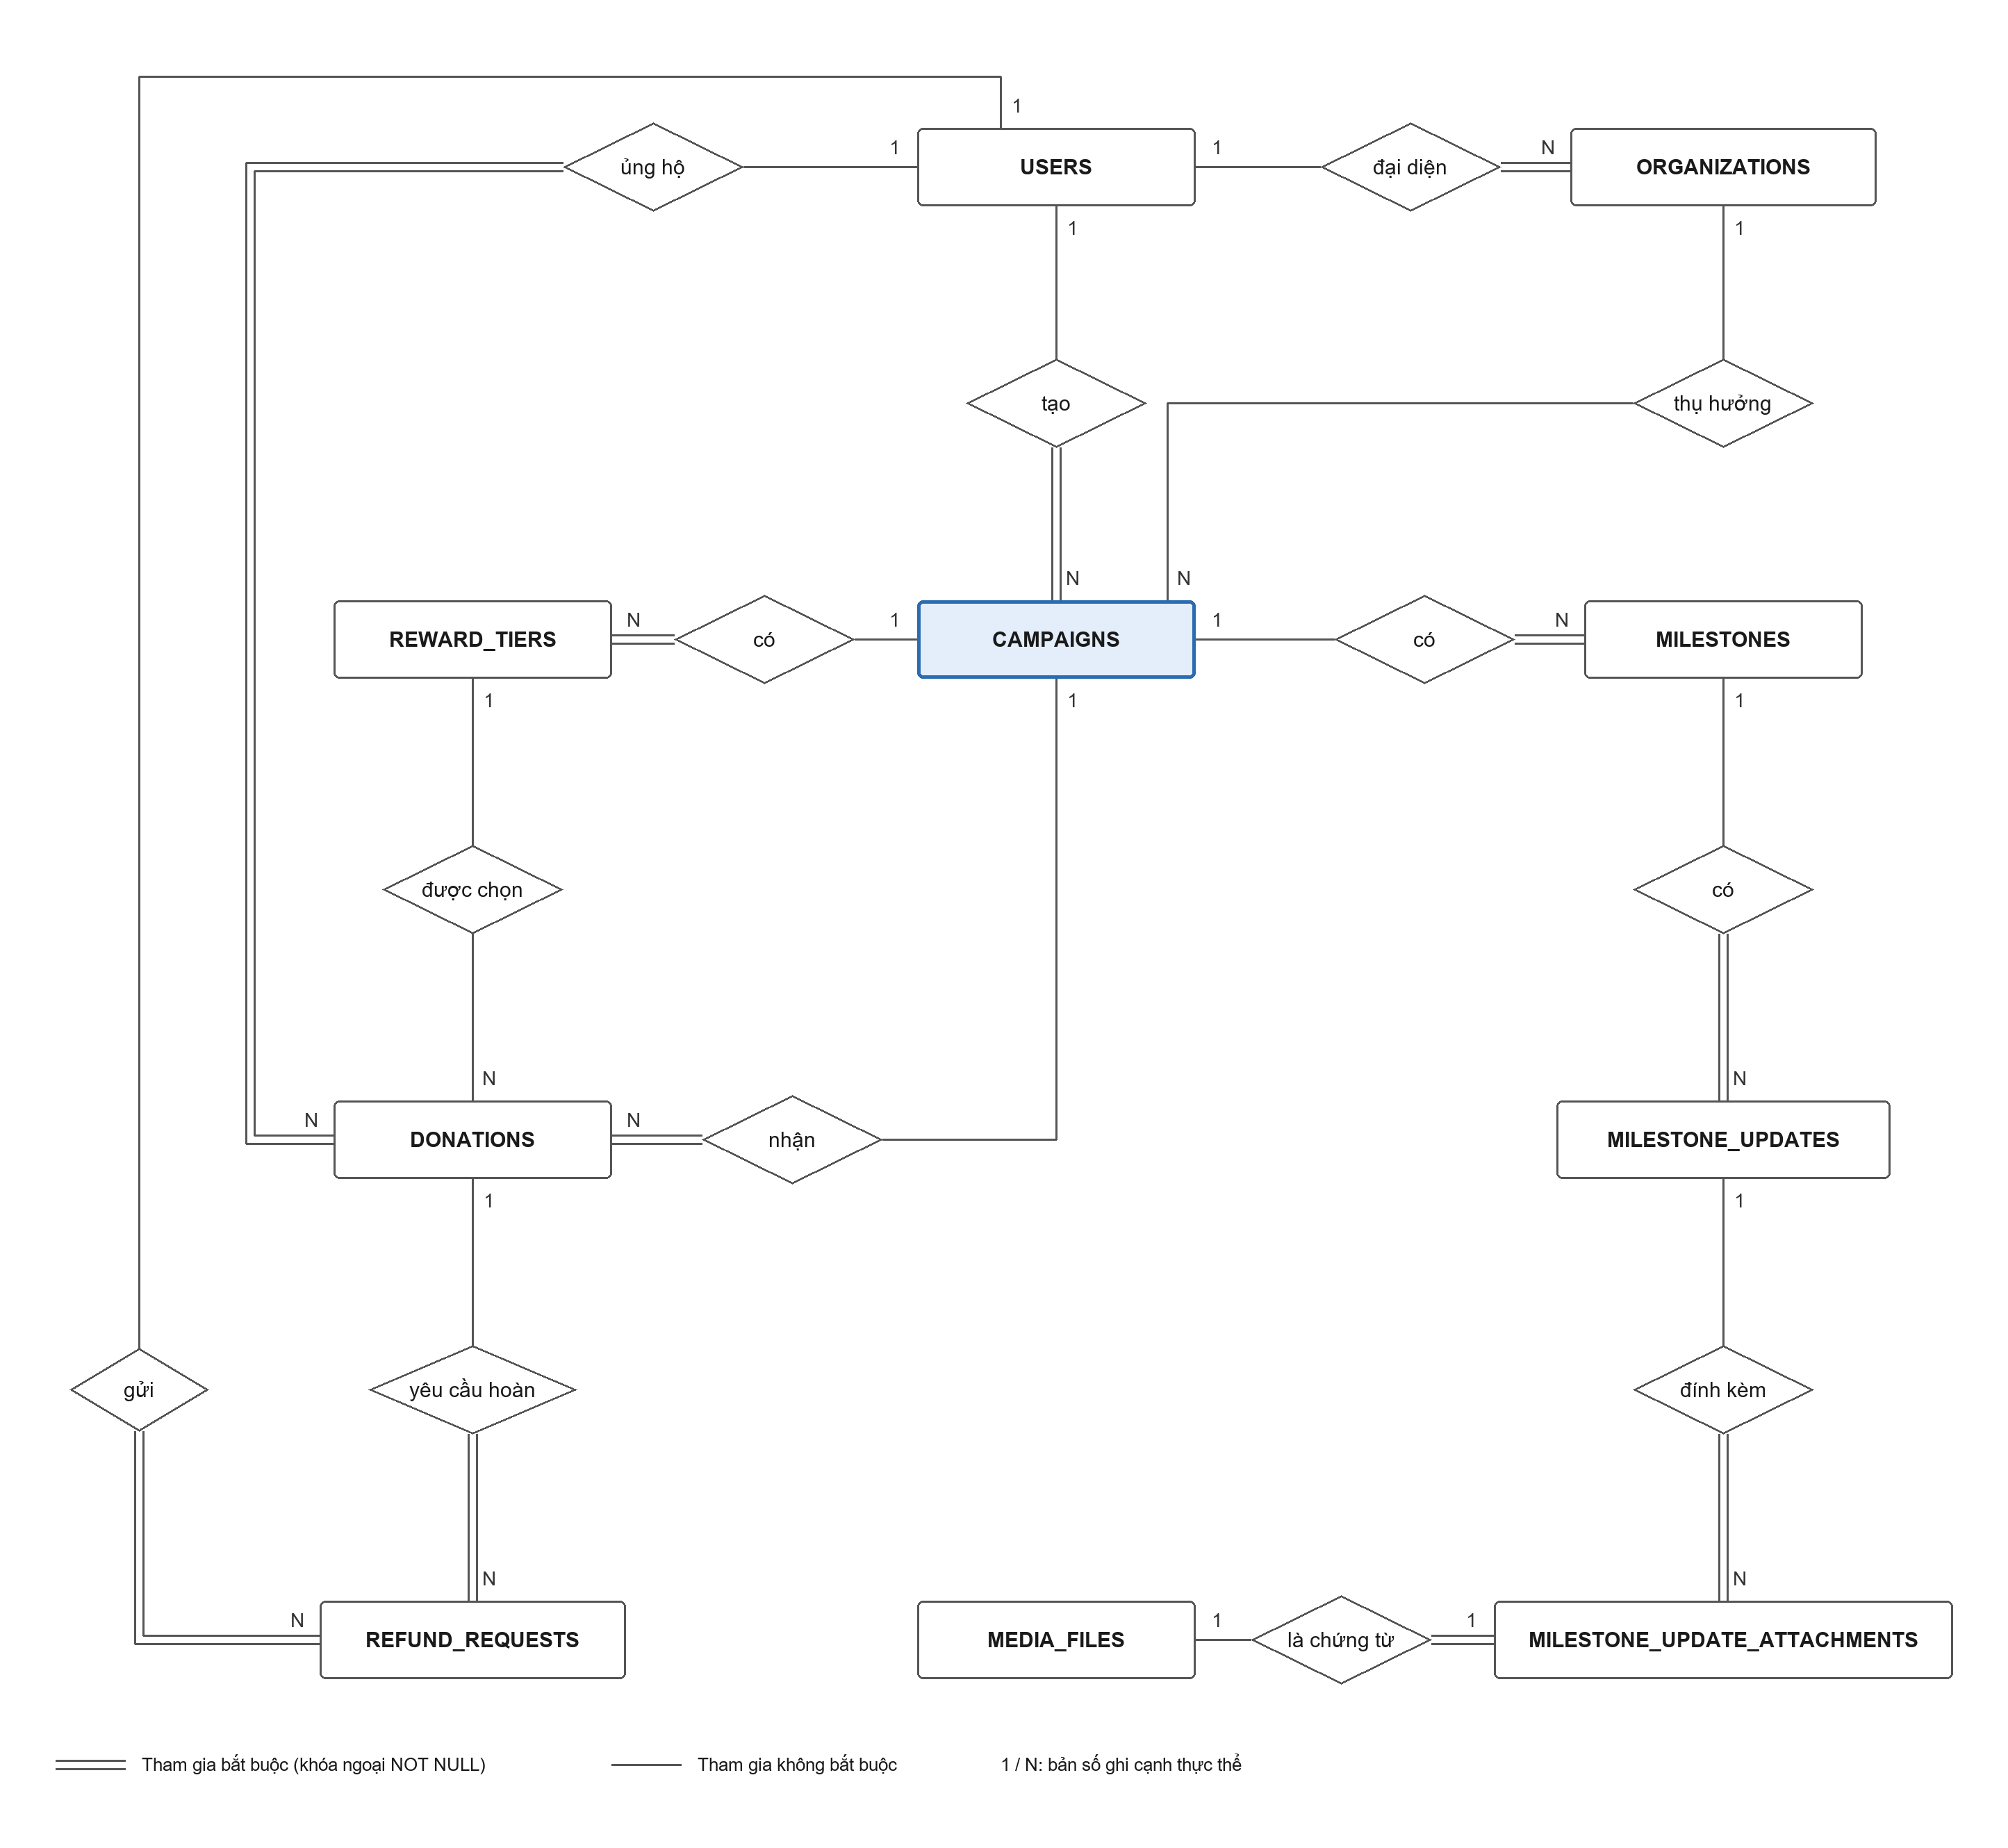
\includegraphics[width=\textwidth,height=0.72\textheight,keepaspectratio]{image/MoHinhQuanHe_GopMam.png}
    \caption{Mô hình quan hệ lõi (ký hiệu Chen)}
    \label{fig:mo_hinh_quan_he}
\end{figure}

Hình gồm các thực thể lõi của luồng gây quỹ (kể cả tổ chức thụ hưởng), ủng hộ, hoàn tiền và giải ngân; nét đôi là phía tham gia bắt buộc (khóa ngoại NOT NULL). Đủ 24 thực thể và 37 quan hệ được đặc tả ở Chương 2 và Chương 3.

	\newpage

	\section{CÁC THỰC THỂ (ENTITIES)}\label{sec:chuong2}

Mọi khóa chính là UUID dạng CHAR(36) do ứng dụng sinh, trừ hai ngoại lệ ghi rõ ở 2.4 và 2.7. Cột created\_\allowbreak{}at, updated\_\allowbreak{}at kiểu DATETIME(6), mặc định CURRENT\_\allowbreak{}TIMESTAMP(6); updated\_\allowbreak{}at tự cập nhật khi sửa bản ghi.

\subsection{USERS (Người dùng)}

\textbf{Mục đích:} Lưu tài khoản đăng nhập và hồ sơ người dùng. Một tài khoản có thể vừa ủng hộ vừa làm chủ chiến dịch; quyền quản trị phân biệt bằng role.

{\small
\begin{longtable}{|P{3.2cm}|P{2.8cm}|P{2.2cm}|p{5.4cm}|}
    \caption{Thuộc tính của bảng USERS}
    \label{tab:users} \\
    \hline
    \textbf{Thuộc tính} & \textbf{Kiểu dữ liệu} & \textbf{Ràng buộc} & \textbf{Mô tả} \\
    \hline
    \endfirsthead
    \hline
    \textbf{Thuộc tính} & \textbf{Kiểu dữ liệu} & \textbf{Ràng buộc} & \textbf{Mô tả} \\
    \hline
    \endhead

    \texttt{id} & CHAR(36) & PK & Mã định danh duy nhất \\
    \hline
    \texttt{name} & VARCHAR(100) & NOT NULL & Họ tên hiển thị \\
    \hline
    \texttt{email} & VARCHAR(255) & NOT NULL, UNIQUE & Email đăng nhập \\
    \hline
    \texttt{password\_\allowbreak{}hash} & VARCHAR(255) & NOT NULL & Mật khẩu đã băm, không bao giờ trả ra API; tài khoản tạo bằng Google nhận hash của một mật khẩu ngẫu nhiên, người dùng tự đặt mật khẩu qua chức năng quên mật khẩu \\
    \hline
    \texttt{google\_\allowbreak{}id} & VARCHAR(64) & UNIQUE & Mã tài khoản Google (sub) khi đăng nhập bằng Google; NULL là chưa liên kết. Nhận diện theo cột này nên người dùng đổi email Google vẫn vào đúng tài khoản \\
    \hline
    \texttt{role} & ENUM: user / campaign\_\allowbreak{}owner / admin & NOT NULL & Vai trò, mặc định user \\
    \hline
    \texttt{status} & ENUM: active / inactive / banned & NOT NULL & Trạng thái tài khoản, mặc định active \\
    \hline
    \texttt{avatar} & VARCHAR(255) &  & Đường dẫn ảnh đại diện \\
    \hline
    \texttt{bio} & VARCHAR(500) &  & Giới thiệu ngắn \\
    \hline
    \texttt{phone} & VARCHAR(100) &  & Số điện thoại, chỉ chính chủ và quản trị viên xem được \\
    \hline
    \texttt{organization} & VARCHAR(255) &  & Đơn vị công tác ghi tự do trên hồ sơ cá nhân; không liên quan tới bảng ORGANIZATIONS (mục 2.23) \\
    \hline
    \texttt{email\_\allowbreak{}verified} & TINYINT(1) & NOT NULL & Đã xác minh email, mặc định 0 \\
    \hline
    \texttt{failed\_\allowbreak{}login\_\allowbreak{}count} & INT & NOT NULL & Số lần đăng nhập sai liên tiếp, mặc định 0 \\
    \hline
    \texttt{locked\_\allowbreak{}until} & DATETIME &  & Khóa đăng nhập tạm thời tới thời điểm này \\
    \hline
    \texttt{password\_\allowbreak{}changed\_\allowbreak{}at} & DATETIME &  & JWT phát hành trước thời điểm này bị từ chối \\
    \hline
    \texttt{sessions\_\allowbreak{}revoked\_\allowbreak{}at} & DATETIME &  & Thời điểm đăng xuất khỏi mọi thiết bị \\
    \hline
    \texttt{ai\_\allowbreak{}tracking\_\allowbreak{}consent} & TINYINT(1) & NOT NULL & Đồng ý ghi nhận hành vi cho gợi ý AI, mặc định 0 \\
    \hline
    \texttt{ai\_\allowbreak{}consent\_\allowbreak{}updated\_\allowbreak{}at} & DATETIME &  & Lần cuối đổi lựa chọn đồng ý; NULL là chưa từng quyết định \\
    \hline
    \texttt{created\_\allowbreak{}at} & DATETIME(6) & NOT NULL & Thời điểm tạo \\
    \hline
    \texttt{updated\_\allowbreak{}at} & DATETIME(6) & NOT NULL & Thời điểm cập nhật cuối \\
    \hline
\end{longtable}
}

\textbf{Ràng buộc:}
\begin{itemize}
    \item UNIQUE trên email; UNIQUE trên google\_\allowbreak{}id (cho phép NULL).
\end{itemize}

\subsection{EMAIL\_\allowbreak{}VERIFICATION\_\allowbreak{}TOKENS (Token xác minh email)}

\textbf{Mục đích:} Lưu token một lần gửi qua email để xác minh địa chỉ email.

{\small
\begin{longtable}{|P{3.2cm}|P{2.8cm}|P{2.2cm}|p{5.4cm}|}
    \caption{Thuộc tính của bảng EMAIL\_\allowbreak{}VERIFICATION\_\allowbreak{}TOKENS}
    \label{tab:email_verification_tokens} \\
    \hline
    \textbf{Thuộc tính} & \textbf{Kiểu dữ liệu} & \textbf{Ràng buộc} & \textbf{Mô tả} \\
    \hline
    \endfirsthead
    \hline
    \textbf{Thuộc tính} & \textbf{Kiểu dữ liệu} & \textbf{Ràng buộc} & \textbf{Mô tả} \\
    \hline
    \endhead

    \texttt{id} & CHAR(36) & PK & Mã định danh duy nhất \\
    \hline
    \texttt{user\_\allowbreak{}id} & CHAR(36) & NOT NULL, FK & Người dùng sở hữu token \\
    \hline
    \texttt{token\_\allowbreak{}hash} & CHAR(64) & NOT NULL, UNIQUE & SHA-256 của token; token gốc không được lưu \\
    \hline
    \texttt{expires\_\allowbreak{}at} & DATETIME & NOT NULL & Hạn sử dụng \\
    \hline
    \texttt{used\_\allowbreak{}at} & DATETIME &  & Thời điểm đã dùng; NULL là chưa dùng \\
    \hline
    \texttt{created\_\allowbreak{}at} &  &  &  \\
    \hline
    \texttt{updated\_\allowbreak{}at} & DATETIME(6) & NOT NULL & Thời điểm tạo, cập nhật \\
    \hline
\end{longtable}
}

\textbf{Ràng buộc:}
\begin{itemize}
    \item UNIQUE trên token\_\allowbreak{}hash
    \item INDEX (user\_\allowbreak{}id, created\_\allowbreak{}at)
    \item FK user\_\allowbreak{}id tham chiếu đến users(id), ON DELETE CASCADE
\end{itemize}

\subsection{PASSWORD\_\allowbreak{}RESET\_\allowbreak{}TOKENS (Token đặt lại mật khẩu)}

\textbf{Mục đích:} Lưu token một lần cho chức năng quên mật khẩu.

{\small
\begin{longtable}{|P{3.2cm}|P{2.8cm}|P{2.2cm}|p{5.4cm}|}
    \caption{Thuộc tính của bảng PASSWORD\_\allowbreak{}RESET\_\allowbreak{}TOKENS}
    \label{tab:password_reset_tokens} \\
    \hline
    \textbf{Thuộc tính} & \textbf{Kiểu dữ liệu} & \textbf{Ràng buộc} & \textbf{Mô tả} \\
    \hline
    \endfirsthead
    \hline
    \textbf{Thuộc tính} & \textbf{Kiểu dữ liệu} & \textbf{Ràng buộc} & \textbf{Mô tả} \\
    \hline
    \endhead

    \texttt{id} & CHAR(36) & PK & Mã định danh duy nhất \\
    \hline
    \texttt{user\_\allowbreak{}id} & CHAR(36) & NOT NULL, FK & Người dùng yêu cầu \\
    \hline
    \texttt{token\_\allowbreak{}hash} & CHAR(64) & NOT NULL, UNIQUE & SHA-256 của token \\
    \hline
    \texttt{expires\_\allowbreak{}at} & DATETIME & NOT NULL & Hạn sử dụng \\
    \hline
    \texttt{used\_\allowbreak{}at} & DATETIME &  & Thời điểm đã dùng \\
    \hline
    \texttt{requested\_\allowbreak{}ip} & VARCHAR(45) &  & IP gửi yêu cầu (IPv4/IPv6) \\
    \hline
    \texttt{created\_\allowbreak{}at} &  &  &  \\
    \hline
    \texttt{updated\_\allowbreak{}at} & DATETIME(6) & NOT NULL & Thời điểm tạo, cập nhật \\
    \hline
\end{longtable}
}

\textbf{Ràng buộc:}
\begin{itemize}
    \item UNIQUE trên token\_\allowbreak{}hash
    \item INDEX (user\_\allowbreak{}id, created\_\allowbreak{}at)
    \item FK user\_\allowbreak{}id tham chiếu đến users(id), ON DELETE CASCADE
\end{itemize}

\subsection{REVOKED\_\allowbreak{}TOKENS (Token đã thu hồi)}

\textbf{Mục đích:} Danh sách đen JWT đã đăng xuất, giữ tới khi token tự hết hạn.

{\small
\begin{longtable}{|P{3.2cm}|P{2.8cm}|P{2.2cm}|p{5.4cm}|}
    \caption{Thuộc tính của bảng REVOKED\_\allowbreak{}TOKENS}
    \label{tab:revoked_tokens} \\
    \hline
    \textbf{Thuộc tính} & \textbf{Kiểu dữ liệu} & \textbf{Ràng buộc} & \textbf{Mô tả} \\
    \hline
    \endfirsthead
    \hline
    \textbf{Thuộc tính} & \textbf{Kiểu dữ liệu} & \textbf{Ràng buộc} & \textbf{Mô tả} \\
    \hline
    \endhead

    \texttt{jti} & CHAR(36) & PK & Mã định danh của JWT \\
    \hline
    \texttt{user\_\allowbreak{}id} & CHAR(36) & NOT NULL, FK & Chủ token \\
    \hline
    \texttt{expires\_\allowbreak{}at} & DATETIME & NOT NULL & Thời điểm JWT hết hạn, sau đó có thể xóa bản ghi \\
    \hline
    \texttt{created\_\allowbreak{}at} & DATETIME(6) & NOT NULL & Thời điểm đăng xuất \\
    \hline
\end{longtable}
}

\textbf{Ràng buộc:}
\begin{itemize}
    \item Khóa chính là jti, không có cột id và updated\_\allowbreak{}at
    \item INDEX expires\_\allowbreak{}at để dọn bản ghi hết hạn
    \item FK user\_\allowbreak{}id tham chiếu đến users(id), ON DELETE CASCADE
\end{itemize}

\subsection{CAMPAIGNS (Chiến dịch)}

\textbf{Mục đích:} Quản lý chiến dịch gây quỹ và vòng đời từ nháp, kiểm duyệt, gây quỹ đến kết thúc.

{\small
\begin{longtable}{|P{3.2cm}|P{2.8cm}|P{2.2cm}|p{5.4cm}|}
    \caption{Thuộc tính của bảng CAMPAIGNS}
    \label{tab:campaigns} \\
    \hline
    \textbf{Thuộc tính} & \textbf{Kiểu dữ liệu} & \textbf{Ràng buộc} & \textbf{Mô tả} \\
    \hline
    \endfirsthead
    \hline
    \textbf{Thuộc tính} & \textbf{Kiểu dữ liệu} & \textbf{Ràng buộc} & \textbf{Mô tả} \\
    \hline
    \endhead

    \texttt{id} & CHAR(36) & PK & Mã định danh duy nhất \\
    \hline
    \texttt{title} & VARCHAR(200) & NOT NULL & Tên chiến dịch \\
    \hline
    \texttt{description} & MEDIUMTEXT & NOT NULL & Nội dung mô tả dạng HTML soạn bằng trình soạn thảo định dạng, được làm sạch ở server trước khi lưu \\
    \hline
    \texttt{category} & VARCHAR(100) & NOT NULL & Tên danh mục, lấy từ categories.name (tham chiếu logic, không có FK) \\
    \hline
    \texttt{owner\_\allowbreak{}id} & CHAR(36) & NOT NULL, FK & Chủ chiến dịch \\
    \hline
    \texttt{organization\_\allowbreak{}id} & CHAR(36) & FK & Tổ chức thụ hưởng khi gây quỹ cho một tổ chức đã xác minh; NULL là gây quỹ cho dự án của chính chủ chiến dịch \\
    \hline
    \texttt{goal\_\allowbreak{}amount} & DECIMAL(15,2) & NOT NULL & Mục tiêu gây quỹ \\
    \hline
    \texttt{current\_\allowbreak{}amount} & DECIMAL(15,2) & NOT NULL & Số tiền đã gây được, mặc định 0, chỉ cộng từ giao dịch đã xác minh \\
    \hline
    \texttt{start\_\allowbreak{}date} & DATETIME & NOT NULL & Ngày bắt đầu \\
    \hline
    \texttt{end\_\allowbreak{}date} & DATETIME & NOT NULL & Ngày kết thúc \\
    \hline
    \texttt{status} & ENUM & NOT NULL & draft / pending / approved / rejected / needs\_\allowbreak{}info / active / paused / success / failed / cancelled / ended, mặc định draft \\
    \hline
    \texttt{submitted\_\allowbreak{}at} & DATETIME &  & Lần gửi (lại) duyệt gần nhất; hàng chờ kiểm duyệt xếp theo cột này \\
    \hline
    \texttt{is\_\allowbreak{}featured} & TINYINT(1) & NOT NULL & Được quản trị viên chọn nổi bật trên trang chủ, mặc định 0 \\
    \hline
    \texttt{featured\_\allowbreak{}at} & DATETIME &  & Thời điểm được chọn nổi bật, dùng để sắp xếp \\
    \hline
    \texttt{image\_\allowbreak{}url} & VARCHAR(500) &  & Ảnh đại diện \\
    \hline
    \texttt{video\_\allowbreak{}url} & VARCHAR(500) &  & Video giới thiệu \\
    \hline
    \texttt{location} & VARCHAR(255) &  & Địa điểm \\
    \hline
    \texttt{backer\_\allowbreak{}count} & INT & NOT NULL & Số người ủng hộ, mặc định 0 \\
    \hline
    \texttt{view\_\allowbreak{}count} & INT & NOT NULL & Tổng lượt xem tích lũy, mặc định 0 \\
    \hline
    \texttt{rejection\_\allowbreak{}reason} & TEXT &  & Lý do từ chối hoặc yêu cầu bổ sung khi kiểm duyệt \\
    \hline
    \texttt{created\_\allowbreak{}at} &  &  &  \\
    \hline
    \texttt{updated\_\allowbreak{}at} & DATETIME(6) & NOT NULL & Thời điểm tạo, cập nhật \\
    \hline
\end{longtable}
}

\textbf{Ràng buộc:}
\begin{itemize}
    \item FK owner\_\allowbreak{}id tham chiếu đến users(id); FK organization\_\allowbreak{}id tham chiếu đến organizations(id)
    \item INDEX status, INDEX category, INDEX (is\_\allowbreak{}featured, featured\_\allowbreak{}at), INDEX organization\_\allowbreak{}id
\end{itemize}

\subsection{CATEGORIES (Danh mục lĩnh vực)}

\textbf{Mục đích:} Danh mục lĩnh vực chiến dịch do quản trị viên quản lý. Migration tạo sẵn 6 danh mục: Giáo dục, Môi trường, Nông nghiệp, Y tế, Khởi nghiệp, Công nghệ.

{\small
\begin{longtable}{|P{3.2cm}|P{2.8cm}|P{2.2cm}|p{5.4cm}|}
    \caption{Thuộc tính của bảng CATEGORIES}
    \label{tab:categories} \\
    \hline
    \textbf{Thuộc tính} & \textbf{Kiểu dữ liệu} & \textbf{Ràng buộc} & \textbf{Mô tả} \\
    \hline
    \endfirsthead
    \hline
    \textbf{Thuộc tính} & \textbf{Kiểu dữ liệu} & \textbf{Ràng buộc} & \textbf{Mô tả} \\
    \hline
    \endhead

    \texttt{id} & CHAR(36) & PK & Mã định danh duy nhất \\
    \hline
    \texttt{name} & VARCHAR(100) & NOT NULL, UNIQUE & Tên danh mục \\
    \hline
    \texttt{description} & VARCHAR(300) &  & Mô tả ngắn \\
    \hline
    \texttt{sort\_\allowbreak{}order} & INT & NOT NULL & Thứ tự hiển thị, mặc định 0 \\
    \hline
    \texttt{is\_\allowbreak{}active} & TINYINT(1) & NOT NULL & Đang dùng, mặc định 1; tắt thì không nhận chiến dịch mới \\
    \hline
    \texttt{created\_\allowbreak{}at} &  &  &  \\
    \hline
    \texttt{updated\_\allowbreak{}at} & DATETIME(6) & NOT NULL & Thời điểm tạo, cập nhật \\
    \hline
\end{longtable}
}

\textbf{Ràng buộc:}
\begin{itemize}
    \item UNIQUE trên name; không có khóa ngoại.
\end{itemize}

\subsection{CAMPAIGN\_\allowbreak{}VIEW\_\allowbreak{}DAILY (Lượt xem theo ngày)}

\textbf{Mục đích:} Đếm lượt xem chiến dịch theo ngày (UTC) để chủ dự án xem diễn biến và tính tỷ lệ chuyển đổi.

{\small
\begin{longtable}{|P{3.2cm}|P{2.8cm}|P{2.2cm}|p{5.4cm}|}
    \caption{Thuộc tính của bảng CAMPAIGN\_\allowbreak{}VIEW\_\allowbreak{}DAILY}
    \label{tab:campaign_view_daily} \\
    \hline
    \textbf{Thuộc tính} & \textbf{Kiểu dữ liệu} & \textbf{Ràng buộc} & \textbf{Mô tả} \\
    \hline
    \endfirsthead
    \hline
    \textbf{Thuộc tính} & \textbf{Kiểu dữ liệu} & \textbf{Ràng buộc} & \textbf{Mô tả} \\
    \hline
    \endhead

    \texttt{campaign\_\allowbreak{}id} & CHAR(36) & NOT NULL, PK, FK & Chiến dịch \\
    \hline
    \texttt{view\_\allowbreak{}date} & DATE & NOT NULL, PK & Ngày thống kê \\
    \hline
    \texttt{views} & INT & NOT NULL & Số lượt xem trong ngày, mặc định 0 \\
    \hline
\end{longtable}
}

\textbf{Ràng buộc:}
\begin{itemize}
    \item PRIMARY KEY (campaign\_\allowbreak{}id, view\_\allowbreak{}date); bảng không có id, created\_\allowbreak{}at, updated\_\allowbreak{}at
    \item FK campaign\_\allowbreak{}id tham chiếu đến campaigns(id), ON DELETE CASCADE
\end{itemize}

\subsection{MILESTONES (Mốc tiến độ)}

\textbf{Mục đích:} Các mốc sử dụng quỹ của chiến dịch, giúp người ủng hộ theo dõi việc giải ngân.

{\small
\begin{longtable}{|P{3.2cm}|P{2.8cm}|P{2.2cm}|p{5.4cm}|}
    \caption{Thuộc tính của bảng MILESTONES}
    \label{tab:milestones} \\
    \hline
    \textbf{Thuộc tính} & \textbf{Kiểu dữ liệu} & \textbf{Ràng buộc} & \textbf{Mô tả} \\
    \hline
    \endfirsthead
    \hline
    \textbf{Thuộc tính} & \textbf{Kiểu dữ liệu} & \textbf{Ràng buộc} & \textbf{Mô tả} \\
    \hline
    \endhead

    \texttt{id} & CHAR(36) & PK & Mã định danh duy nhất \\
    \hline
    \texttt{campaign\_\allowbreak{}id} & CHAR(36) & NOT NULL, FK & Chiến dịch \\
    \hline
    \texttt{title} & VARCHAR(200) & NOT NULL & Tên mốc \\
    \hline
    \texttt{description} & TEXT &  & Mô tả \\
    \hline
    \texttt{target\_\allowbreak{}date} & DATETIME &  & Ngày dự kiến hoàn thành \\
    \hline
    \texttt{budget} & DECIMAL(15,2) &  & Ngân sách dự kiến \\
    \hline
    \texttt{sort\_\allowbreak{}order} & INT & NOT NULL & Thứ tự hiển thị, mặc định 0 \\
    \hline
    \texttt{is\_\allowbreak{}completed} & TINYINT(1) & NOT NULL & Đã hoàn thành, mặc định 0 \\
    \hline
    \texttt{completed\_\allowbreak{}at} & DATETIME &  & Thời điểm hoàn thành \\
    \hline
    \texttt{overdue\_\allowbreak{}notified\_\allowbreak{}at} & DATETIME &  & Lần cuối nhắc chủ dự án mốc quá hạn (tối đa 7 ngày/lần); đặt lại NULL khi đổi hạn \\
    \hline
    \texttt{created\_\allowbreak{}at} &  &  &  \\
    \hline
    \texttt{updated\_\allowbreak{}at} & DATETIME(6) & NOT NULL & Thời điểm tạo, cập nhật \\
    \hline
\end{longtable}
}

\textbf{Ràng buộc:}
\begin{itemize}
    \item FK campaign\_\allowbreak{}id tham chiếu đến campaigns(id).
\end{itemize}

\subsection{MILESTONE\_\allowbreak{}UPDATES (Cập nhật tiến độ)}

\textbf{Mục đích:} Bài cập nhật cho từng mốc gồm nội dung, hình ảnh và khoản chi.

{\small
\begin{longtable}{|P{3.2cm}|P{2.8cm}|P{2.2cm}|p{5.4cm}|}
    \caption{Thuộc tính của bảng MILESTONE\_\allowbreak{}UPDATES}
    \label{tab:milestone_updates} \\
    \hline
    \textbf{Thuộc tính} & \textbf{Kiểu dữ liệu} & \textbf{Ràng buộc} & \textbf{Mô tả} \\
    \hline
    \endfirsthead
    \hline
    \textbf{Thuộc tính} & \textbf{Kiểu dữ liệu} & \textbf{Ràng buộc} & \textbf{Mô tả} \\
    \hline
    \endhead

    \texttt{id} & CHAR(36) & PK & Mã định danh duy nhất \\
    \hline
    \texttt{milestone\_\allowbreak{}id} & CHAR(36) & NOT NULL, FK & Mốc tiến độ \\
    \hline
    \texttt{content} & TEXT & NOT NULL & Nội dung cập nhật \\
    \hline
    \texttt{image\_\allowbreak{}url} & VARCHAR(500) &  & Ảnh minh họa \\
    \hline
    \texttt{expense\_\allowbreak{}amount} & DECIMAL(15,2) &  & Số tiền đã chi \\
    \hline
    \texttt{created\_\allowbreak{}at} &  &  &  \\
    \hline
    \texttt{updated\_\allowbreak{}at} & DATETIME(6) & NOT NULL & Thời điểm tạo, cập nhật \\
    \hline
\end{longtable}
}

\textbf{Ràng buộc:}
\begin{itemize}
    \item FK milestone\_\allowbreak{}id tham chiếu đến milestones(id).
\end{itemize}

\subsection{MILESTONE\_\allowbreak{}UPDATE\_\allowbreak{}ATTACHMENTS (Chứng từ chi tiêu)}

\textbf{Mục đích:} Gắn ảnh hóa đơn, biên lai (tệp MEDIA\_\allowbreak{}FILES có purpose = expense\_\allowbreak{}receipt) vào bài cập nhật tiến độ để minh bạch khoản chi.

{\small
\begin{longtable}{|P{3.2cm}|P{2.8cm}|P{2.2cm}|p{5.4cm}|}
    \caption{Thuộc tính của bảng MILESTONE\_\allowbreak{}UPDATE\_\allowbreak{}ATTACHMENTS}
    \label{tab:milestone_update_attachments} \\
    \hline
    \textbf{Thuộc tính} & \textbf{Kiểu dữ liệu} & \textbf{Ràng buộc} & \textbf{Mô tả} \\
    \hline
    \endfirsthead
    \hline
    \textbf{Thuộc tính} & \textbf{Kiểu dữ liệu} & \textbf{Ràng buộc} & \textbf{Mô tả} \\
    \hline
    \endhead

    \texttt{id} & CHAR(36) & PK & Mã định danh duy nhất \\
    \hline
    \texttt{milestone\_\allowbreak{}update\_\allowbreak{}id} & CHAR(36) & NOT NULL, FK & Bài cập nhật chứa chứng từ \\
    \hline
    \texttt{media\_\allowbreak{}file\_\allowbreak{}id} & CHAR(36) & NOT NULL, UNIQUE, FK & Tệp chứng từ đã tải lên \\
    \hline
    \texttt{url} & VARCHAR(500) & NOT NULL & Đường dẫn công khai của chứng từ \\
    \hline
    \texttt{caption} & VARCHAR(200) &  & Chú thích khoản chi \\
    \hline
    \texttt{sort\_\allowbreak{}order} & INT & NOT NULL & Thứ tự hiển thị, mặc định 0 \\
    \hline
    \texttt{created\_\allowbreak{}at} &  &  &  \\
    \hline
    \texttt{updated\_\allowbreak{}at} & DATETIME(6) & NOT NULL & Thời điểm tạo, cập nhật \\
    \hline
\end{longtable}
}

\textbf{Ràng buộc:}
\begin{itemize}
    \item UNIQUE trên media\_\allowbreak{}file\_\allowbreak{}id: một chứng từ không dùng lại cho nhiều khoản chi
    \item INDEX (milestone\_\allowbreak{}update\_\allowbreak{}id, sort\_\allowbreak{}order)
    \item FK milestone\_\allowbreak{}update\_\allowbreak{}id tham chiếu đến milestone\_\allowbreak{}updates(id), ON DELETE CASCADE
    \item FK media\_\allowbreak{}file\_\allowbreak{}id tham chiếu đến media\_\allowbreak{}files(id)
\end{itemize}

\subsection{MILESTONE\_\allowbreak{}REVISIONS (Lịch sử thay đổi mốc)}

\textbf{Mục đích:} Ghi lại mỗi lần chủ dự án sửa mốc sau khi chiến dịch đã phát hành, kèm lý do bắt buộc, công khai cho người ủng hộ.

{\small
\begin{longtable}{|P{3.2cm}|P{2.8cm}|P{2.2cm}|p{5.4cm}|}
    \caption{Thuộc tính của bảng MILESTONE\_\allowbreak{}REVISIONS}
    \label{tab:milestone_revisions} \\
    \hline
    \textbf{Thuộc tính} & \textbf{Kiểu dữ liệu} & \textbf{Ràng buộc} & \textbf{Mô tả} \\
    \hline
    \endfirsthead
    \hline
    \textbf{Thuộc tính} & \textbf{Kiểu dữ liệu} & \textbf{Ràng buộc} & \textbf{Mô tả} \\
    \hline
    \endhead

    \texttt{id} & CHAR(36) & PK & Mã định danh duy nhất \\
    \hline
    \texttt{milestone\_\allowbreak{}id} & CHAR(36) & NOT NULL, FK & Mốc bị thay đổi \\
    \hline
    \texttt{changed\_\allowbreak{}by} & CHAR(36) & NOT NULL, FK & Người thực hiện thay đổi \\
    \hline
    \texttt{reason} & VARCHAR(500) & NOT NULL & Lý do thay đổi \\
    \hline
    \texttt{old\_\allowbreak{}values} & TEXT & NOT NULL & Giá trị trước khi sửa, dạng chuỗi JSON \\
    \hline
    \texttt{new\_\allowbreak{}values} & TEXT & NOT NULL & Giá trị sau khi sửa, dạng chuỗi JSON \\
    \hline
    \texttt{created\_\allowbreak{}at} &  &  &  \\
    \hline
    \texttt{updated\_\allowbreak{}at} & DATETIME(6) & NOT NULL & Thời điểm tạo, cập nhật \\
    \hline
\end{longtable}
}

\textbf{Ràng buộc:}
\begin{itemize}
    \item INDEX (milestone\_\allowbreak{}id, created\_\allowbreak{}at)
    \item FK milestone\_\allowbreak{}id tham chiếu đến milestones(id), ON DELETE CASCADE
    \item FK changed\_\allowbreak{}by tham chiếu đến users(id)
\end{itemize}

\subsection{REWARD\_\allowbreak{}TIERS (Mức quà tặng)}

\textbf{Mục đích:} Các mức ủng hộ kèm phần quà do chủ chiến dịch thiết lập.

{\small
\begin{longtable}{|P{3.2cm}|P{2.8cm}|P{2.2cm}|p{5.4cm}|}
    \caption{Thuộc tính của bảng REWARD\_\allowbreak{}TIERS}
    \label{tab:reward_tiers} \\
    \hline
    \textbf{Thuộc tính} & \textbf{Kiểu dữ liệu} & \textbf{Ràng buộc} & \textbf{Mô tả} \\
    \hline
    \endfirsthead
    \hline
    \textbf{Thuộc tính} & \textbf{Kiểu dữ liệu} & \textbf{Ràng buộc} & \textbf{Mô tả} \\
    \hline
    \endhead

    \texttt{id} & CHAR(36) & PK & Mã định danh duy nhất \\
    \hline
    \texttt{campaign\_\allowbreak{}id} & CHAR(36) & NOT NULL, FK & Chiến dịch \\
    \hline
    \texttt{title} & VARCHAR(120) & NOT NULL & Tên mức quà \\
    \hline
    \texttt{description} & TEXT & NOT NULL & Mô tả phần quà \\
    \hline
    \texttt{min\_\allowbreak{}amount} & DECIMAL(15,2) & NOT NULL & Số tiền ủng hộ tối thiểu \\
    \hline
    \texttt{quantity\_\allowbreak{}limit} & INT &  & Số suất tối đa; NULL là không giới hạn \\
    \hline
    \texttt{claimed\_\allowbreak{}count} & INT & NOT NULL & Số suất đã nhận, mặc định 0, chỉ tăng khi thanh toán được xác nhận \\
    \hline
    \texttt{estimated\_\allowbreak{}delivery} & DATE &  & Ngày dự kiến giao quà \\
    \hline
    \texttt{sort\_\allowbreak{}order} & INT & NOT NULL & Thứ tự hiển thị, mặc định 0 \\
    \hline
    \texttt{is\_\allowbreak{}active} & TINYINT(1) & NOT NULL & Đang mở, mặc định 1 \\
    \hline
    \texttt{created\_\allowbreak{}at} &  &  &  \\
    \hline
    \texttt{updated\_\allowbreak{}at} & DATETIME(6) & NOT NULL & Thời điểm tạo, cập nhật \\
    \hline
    \texttt{deleted\_\allowbreak{}at} & DATETIME(6) &  & Thời điểm xóa mềm \\
    \hline
\end{longtable}
}

\textbf{Ràng buộc:}
\begin{itemize}
    \item CHECK min\_\allowbreak{}amount \textgreater{} 0
    \item CHECK quantity\_\allowbreak{}limit IS NULL OR claimed\_\allowbreak{}count \textless{}= quantity\_\allowbreak{}limit
    \item INDEX (campaign\_\allowbreak{}id, sort\_\allowbreak{}order)
    \item FK campaign\_\allowbreak{}id tham chiếu đến campaigns(id)
\end{itemize}

\subsection{MEDIA\_\allowbreak{}FILES (Tệp đa phương tiện)}

\textbf{Mục đích:} Quản lý ảnh người dùng tải lên: ảnh chiến dịch, ảnh tiến độ, avatar, ảnh chứng từ chi tiêu, chứng từ hoàn tiền, logo và giấy phép tổ chức.

{\small
\begin{longtable}{|P{3.2cm}|P{2.8cm}|P{2.2cm}|p{5.4cm}|}
    \caption{Thuộc tính của bảng MEDIA\_\allowbreak{}FILES}
    \label{tab:media_files} \\
    \hline
    \textbf{Thuộc tính} & \textbf{Kiểu dữ liệu} & \textbf{Ràng buộc} & \textbf{Mô tả} \\
    \hline
    \endfirsthead
    \hline
    \textbf{Thuộc tính} & \textbf{Kiểu dữ liệu} & \textbf{Ràng buộc} & \textbf{Mô tả} \\
    \hline
    \endhead

    \texttt{id} & CHAR(36) & PK & Mã định danh duy nhất \\
    \hline
    \texttt{owner\_\allowbreak{}id} & CHAR(36) & NOT NULL, FK & Người tải lên \\
    \hline
    \texttt{storage\_\allowbreak{}key} & VARCHAR(120) & NOT NULL, UNIQUE & Khóa trong kho lưu trữ do server sinh, ví dụ campaigns/\textless{}uuid\textgreater{}.webp \\
    \hline
    \texttt{mime\_\allowbreak{}type} & VARCHAR(50) & NOT NULL & Kiểu MIME \\
    \hline
    \texttt{size\_\allowbreak{}bytes} & INT & NOT NULL & Dung lượng \\
    \hline
    \texttt{purpose} & ENUM: campaign\_\allowbreak{}image / progress\_\allowbreak{}image / avatar / expense\_\allowbreak{}receipt / refund\_\allowbreak{}proof / organization\_\allowbreak{}logo / organization\_\allowbreak{}document & NOT NULL & Mục đích sử dụng; refund\_\allowbreak{}proof chỉ quản trị viên tải lên; organization\_\allowbreak{}document là ảnh giấy phép, chỉ người đại diện và quản trị viên xem \\
    \hline
    \texttt{original\_\allowbreak{}name} & VARCHAR(255) &  & Tên file gốc, chỉ để hiển thị \\
    \hline
    \texttt{created\_\allowbreak{}at} &  &  &  \\
    \hline
    \texttt{updated\_\allowbreak{}at} & DATETIME(6) & NOT NULL & Thời điểm tạo, cập nhật \\
    \hline
    \texttt{deleted\_\allowbreak{}at} & DATETIME(6) &  & Thời điểm xóa mềm \\
    \hline
\end{longtable}
}

\textbf{Ràng buộc:}
\begin{itemize}
    \item UNIQUE trên storage\_\allowbreak{}key
    \item INDEX (owner\_\allowbreak{}id, created\_\allowbreak{}at)
    \item FK owner\_\allowbreak{}id tham chiếu đến users(id)
\end{itemize}

\subsection{DONATIONS (Khoản ủng hộ)}

\textbf{Mục đích:} Ghi nhận giao dịch ủng hộ (qua cổng thanh toán hoặc chuyển khoản VietQR đối soát bằng SePay) và trạng thái của giao dịch.

{\small
\begin{longtable}{|P{3.2cm}|P{2.8cm}|P{2.2cm}|p{5.4cm}|}
    \caption{Thuộc tính của bảng DONATIONS}
    \label{tab:donations} \\
    \hline
    \textbf{Thuộc tính} & \textbf{Kiểu dữ liệu} & \textbf{Ràng buộc} & \textbf{Mô tả} \\
    \hline
    \endfirsthead
    \hline
    \textbf{Thuộc tính} & \textbf{Kiểu dữ liệu} & \textbf{Ràng buộc} & \textbf{Mô tả} \\
    \hline
    \endhead

    \texttt{id} & CHAR(36) & PK & Mã định danh duy nhất \\
    \hline
    \texttt{user\_\allowbreak{}id} & CHAR(36) & NOT NULL, FK & Người ủng hộ \\
    \hline
    \texttt{campaign\_\allowbreak{}id} & CHAR(36) & NOT NULL, FK & Chiến dịch được ủng hộ \\
    \hline
    \texttt{reward\_\allowbreak{}tier\_\allowbreak{}id} & CHAR(36) & FK & Mức quà đã chọn; NULL là ủng hộ không nhận quà \\
    \hline
    \texttt{amount} & DECIMAL(15,2) & NOT NULL & Số tiền \\
    \hline
    \texttt{currency} & VARCHAR(3) & NOT NULL & Đơn vị tiền, mặc định VND \\
    \hline
    \texttt{status} & ENUM: pending / completed / failed / refunded / expired / cancelled & NOT NULL & Mặc định pending \\
    \hline
    \texttt{payment\_\allowbreak{}method} & VARCHAR(50) &  & Phương thức thanh toán, ví dụ sepay cho chuyển khoản VietQR \\
    \hline
    \texttt{transaction\_\allowbreak{}id} & VARCHAR(255) & UNIQUE & Mã giao dịch của cổng thanh toán \\
    \hline
    \texttt{transfer\_\allowbreak{}code} & VARCHAR(20) & UNIQUE & Mã nội dung chuyển khoản VietQR (ví dụ GM7K2QX9AB) để khớp giao dịch ngân hàng báo về với đúng đơn \\
    \hline
    \texttt{idempotency\_\allowbreak{}key} & VARCHAR(255) & NOT NULL, UNIQUE & Khóa chống ghi nhận trùng \\
    \hline
    \texttt{message} & TEXT &  & Lời nhắn \\
    \hline
    \texttt{is\_\allowbreak{}anonymous} & TINYINT(1) & NOT NULL & Ủng hộ ẩn danh, mặc định 0 \\
    \hline
    \texttt{completed\_\allowbreak{}at} & DATETIME &  & Thời điểm thanh toán thành công \\
    \hline
    \texttt{refunded\_\allowbreak{}at} & DATETIME &  & Thời điểm hoàn tiền \\
    \hline
    \texttt{refund\_\allowbreak{}reference} & VARCHAR(255) &  & Mã hoàn tiền từ cổng thanh toán \\
    \hline
    \texttt{refund\_\allowbreak{}reason} & VARCHAR(500) &  & Lý do hoàn tiền \\
    \hline
    \texttt{refund\_\allowbreak{}method} & VARCHAR(20) &  & gateway (cổng thanh toán hoàn) hoặc manual\_\allowbreak{}transfer (quản trị viên chuyển khoản trả lại, bắt buộc với khoản qua SePay) \\
    \hline
    \texttt{refund\_\allowbreak{}proof\_\allowbreak{}url} & VARCHAR(500) &  & Ảnh chứng từ chuyển khoản hoàn, chỉ với manual\_\allowbreak{}transfer, không bắt buộc \\
    \hline
    \texttt{created\_\allowbreak{}at} &  &  &  \\
    \hline
    \texttt{updated\_\allowbreak{}at} & DATETIME(6) & NOT NULL & Thời điểm tạo, cập nhật \\
    \hline
\end{longtable}
}

\textbf{Ràng buộc:}
\begin{itemize}
    \item UNIQUE trên transaction\_\allowbreak{}id và transfer\_\allowbreak{}code (đều cho phép NULL), UNIQUE trên idempotency\_\allowbreak{}key
    \item INDEX user\_\allowbreak{}id, INDEX campaign\_\allowbreak{}id, INDEX (status, created\_\allowbreak{}at)
    \item FK user\_\allowbreak{}id tham chiếu đến users(id); FK campaign\_\allowbreak{}id tham chiếu đến campaigns(id); FK reward\_\allowbreak{}tier\_\allowbreak{}id tham chiếu đến reward\_\allowbreak{}tiers(id)
\end{itemize}

\subsection{REFUND\_\allowbreak{}REQUESTS (Yêu cầu hoàn tiền)}

\textbf{Mục đích:} Người ủng hộ gửi yêu cầu hoàn tiền, quản trị viên duyệt hoặc từ chối.

{\small
\begin{longtable}{|P{3.2cm}|P{2.8cm}|P{2.2cm}|p{5.4cm}|}
    \caption{Thuộc tính của bảng REFUND\_\allowbreak{}REQUESTS}
    \label{tab:refund_requests} \\
    \hline
    \textbf{Thuộc tính} & \textbf{Kiểu dữ liệu} & \textbf{Ràng buộc} & \textbf{Mô tả} \\
    \hline
    \endfirsthead
    \hline
    \textbf{Thuộc tính} & \textbf{Kiểu dữ liệu} & \textbf{Ràng buộc} & \textbf{Mô tả} \\
    \hline
    \endhead

    \texttt{id} & CHAR(36) & PK & Mã định danh duy nhất \\
    \hline
    \texttt{donation\_\allowbreak{}id} & CHAR(36) & NOT NULL, FK & Khoản ủng hộ cần hoàn \\
    \hline
    \texttt{user\_\allowbreak{}id} & CHAR(36) & NOT NULL, FK & Người yêu cầu \\
    \hline
    \texttt{reason} & TEXT & NOT NULL & Lý do \\
    \hline
    \texttt{bank\_\allowbreak{}name} & VARCHAR(100) &  & Ngân hàng nhận tiền hoàn \\
    \hline
    \texttt{bank\_\allowbreak{}account\_\allowbreak{}number} & VARCHAR(30) &  & Số tài khoản nhận; nhật ký kiểm toán chỉ giữ 4 số cuối \\
    \hline
    \texttt{bank\_\allowbreak{}account\_\allowbreak{}name} & VARCHAR(100) &  & Tên chủ tài khoản \\
    \hline
    \texttt{status} & ENUM: pending / approved / rejected & NOT NULL & Mặc định pending \\
    \hline
    \texttt{admin\_\allowbreak{}notes} & TEXT &  & Ghi chú của quản trị viên \\
    \hline
    \texttt{reviewed\_\allowbreak{}by} & CHAR(36) & FK & Quản trị viên xử lý \\
    \hline
    \texttt{reviewed\_\allowbreak{}at} & DATETIME &  & Thời điểm xử lý \\
    \hline
    \texttt{created\_\allowbreak{}at} &  &  &  \\
    \hline
    \texttt{updated\_\allowbreak{}at} & DATETIME(6) & NOT NULL & Thời điểm tạo, cập nhật \\
    \hline
\end{longtable}
}

\textbf{Ràng buộc:}
\begin{itemize}
    \item INDEX (status, created\_\allowbreak{}at), INDEX (donation\_\allowbreak{}id, status)
    \item Ba cột ngân hàng nhập đủ cả ba hoặc để trống cả ba (kiểm ở tầng dịch vụ); cần khi khoản ủng hộ phải hoàn bằng chuyển khoản thủ công
    \item FK donation\_\allowbreak{}id tham chiếu đến donations(id); FK user\_\allowbreak{}id và reviewed\_\allowbreak{}by tham chiếu đến users(id)
\end{itemize}

\subsection{CAMPAIGN\_\allowbreak{}COMMENTS (Bình luận chiến dịch)}

\textbf{Mục đích:} Bình luận và câu hỏi của cộng đồng trên trang chiến dịch, hỗ trợ trả lời một cấp.

{\small
\begin{longtable}{|P{3.2cm}|P{2.8cm}|P{2.2cm}|p{5.4cm}|}
    \caption{Thuộc tính của bảng CAMPAIGN\_\allowbreak{}COMMENTS}
    \label{tab:campaign_comments} \\
    \hline
    \textbf{Thuộc tính} & \textbf{Kiểu dữ liệu} & \textbf{Ràng buộc} & \textbf{Mô tả} \\
    \hline
    \endfirsthead
    \hline
    \textbf{Thuộc tính} & \textbf{Kiểu dữ liệu} & \textbf{Ràng buộc} & \textbf{Mô tả} \\
    \hline
    \endhead

    \texttt{id} & CHAR(36) & PK & Mã định danh duy nhất \\
    \hline
    \texttt{campaign\_\allowbreak{}id} & CHAR(36) & NOT NULL, FK & Chiến dịch \\
    \hline
    \texttt{user\_\allowbreak{}id} & CHAR(36) & NOT NULL, FK & Người viết \\
    \hline
    \texttt{parent\_\allowbreak{}id} & CHAR(36) & FK & Bình luận gốc được trả lời; NULL là bình luận gốc \\
    \hline
    \texttt{kind} & ENUM: comment / question & NOT NULL & Loại, mặc định comment \\
    \hline
    \texttt{content} & TEXT & NOT NULL & Nội dung \\
    \hline
    \texttt{status} & ENUM: visible / hidden & NOT NULL & Mặc định visible \\
    \hline
    \texttt{hidden\_\allowbreak{}reason} & VARCHAR(500) &  & Lý do ẩn \\
    \hline
    \texttt{hidden\_\allowbreak{}by} & CHAR(36) & FK & Người ẩn bình luận \\
    \hline
    \texttt{hidden\_\allowbreak{}at} & DATETIME &  & Thời điểm ẩn \\
    \hline
    \texttt{created\_\allowbreak{}at} &  &  &  \\
    \hline
    \texttt{updated\_\allowbreak{}at} & DATETIME(6) & NOT NULL & Thời điểm tạo, cập nhật \\
    \hline
    \texttt{deleted\_\allowbreak{}at} & DATETIME(6) &  & Thời điểm xóa mềm \\
    \hline
\end{longtable}
}

\textbf{Ràng buộc:}
\begin{itemize}
    \item INDEX (campaign\_\allowbreak{}id, parent\_\allowbreak{}id, created\_\allowbreak{}at), INDEX (status, created\_\allowbreak{}at)
    \item FK campaign\_\allowbreak{}id tham chiếu đến campaigns(id); FK user\_\allowbreak{}id, hidden\_\allowbreak{}by tham chiếu đến users(id); FK parent\_\allowbreak{}id tham chiếu đến campaign\_\allowbreak{}comments(id)
\end{itemize}

\subsection{CAMPAIGN\_\allowbreak{}FOLLOWS (Theo dõi chiến dịch)}

\textbf{Mục đích:} Bảng trung gian thể hiện người dùng theo dõi chiến dịch để nhận thông báo cập nhật.

{\small
\begin{longtable}{|P{3.2cm}|P{2.8cm}|P{2.2cm}|p{5.4cm}|}
    \caption{Thuộc tính của bảng CAMPAIGN\_\allowbreak{}FOLLOWS}
    \label{tab:campaign_follows} \\
    \hline
    \textbf{Thuộc tính} & \textbf{Kiểu dữ liệu} & \textbf{Ràng buộc} & \textbf{Mô tả} \\
    \hline
    \endfirsthead
    \hline
    \textbf{Thuộc tính} & \textbf{Kiểu dữ liệu} & \textbf{Ràng buộc} & \textbf{Mô tả} \\
    \hline
    \endhead

    \texttt{id} & CHAR(36) & PK & Mã định danh duy nhất \\
    \hline
    \texttt{user\_\allowbreak{}id} & CHAR(36) & NOT NULL, FK & Người theo dõi \\
    \hline
    \texttt{campaign\_\allowbreak{}id} & CHAR(36) & NOT NULL, FK & Chiến dịch được theo dõi \\
    \hline
    \texttt{created\_\allowbreak{}at} &  &  &  \\
    \hline
    \texttt{updated\_\allowbreak{}at} & DATETIME(6) & NOT NULL & Thời điểm tạo, cập nhật \\
    \hline
\end{longtable}
}

\textbf{Ràng buộc:}
\begin{itemize}
    \item UNIQUE (user\_\allowbreak{}id, campaign\_\allowbreak{}id): mỗi người chỉ theo dõi một chiến dịch một lần
    \item INDEX campaign\_\allowbreak{}id
    \item FK user\_\allowbreak{}id tham chiếu đến users(id) và FK campaign\_\allowbreak{}id tham chiếu đến campaigns(id), đều ON DELETE CASCADE
\end{itemize}

\subsection{REPORTS (Báo cáo vi phạm)}

\textbf{Mục đích:} Người dùng báo cáo chiến dịch hoặc bình luận vi phạm; quản trị viên xử lý.

{\small
\begin{longtable}{|P{3.2cm}|P{2.8cm}|P{2.2cm}|p{5.4cm}|}
    \caption{Thuộc tính của bảng REPORTS}
    \label{tab:reports} \\
    \hline
    \textbf{Thuộc tính} & \textbf{Kiểu dữ liệu} & \textbf{Ràng buộc} & \textbf{Mô tả} \\
    \hline
    \endfirsthead
    \hline
    \textbf{Thuộc tính} & \textbf{Kiểu dữ liệu} & \textbf{Ràng buộc} & \textbf{Mô tả} \\
    \hline
    \endhead

    \texttt{id} & CHAR(36) & PK & Mã định danh duy nhất \\
    \hline
    \texttt{reporter\_\allowbreak{}id} & CHAR(36) & NOT NULL, FK & Người báo cáo \\
    \hline
    \texttt{campaign\_\allowbreak{}id} & CHAR(36) & FK & Chiến dịch bị báo cáo \\
    \hline
    \texttt{comment\_\allowbreak{}id} & CHAR(36) & FK & Bình luận bị báo cáo, nếu có \\
    \hline
    \texttt{reason} & ENUM: spam / fraud / inappropriate / misinformation / other & NOT NULL & Lý do \\
    \hline
    \texttt{description} & TEXT & NOT NULL & Mô tả chi tiết \\
    \hline
    \texttt{status} & ENUM: pending / reviewing / resolved / dismissed & NOT NULL & Mặc định pending \\
    \hline
    \texttt{admin\_\allowbreak{}notes} & TEXT &  & Ghi chú xử lý \\
    \hline
    \texttt{resolved\_\allowbreak{}by} & CHAR(36) & FK & Quản trị viên xử lý gần nhất \\
    \hline
    \texttt{resolved\_\allowbreak{}at} & DATETIME &  & Thời điểm xử lý \\
    \hline
    \texttt{campaign\_\allowbreak{}paused} & TINYINT(1) & NOT NULL & Đã tạm dừng chiến dịch khi xử lý, mặc định 0 \\
    \hline
    \texttt{comment\_\allowbreak{}hidden} & TINYINT(1) & NOT NULL & Đã ẩn bình luận khi xử lý, mặc định 0 \\
    \hline
    \texttt{created\_\allowbreak{}at} &  &  &  \\
    \hline
    \texttt{updated\_\allowbreak{}at} & DATETIME(6) & NOT NULL & Thời điểm tạo, cập nhật \\
    \hline
\end{longtable}
}

\textbf{Ràng buộc:}
\begin{itemize}
    \item INDEX (status, created\_\allowbreak{}at), INDEX (campaign\_\allowbreak{}id, reporter\_\allowbreak{}id)
    \item FK reporter\_\allowbreak{}id, resolved\_\allowbreak{}by tham chiếu đến users(id); FK campaign\_\allowbreak{}id tham chiếu đến campaigns(id); FK comment\_\allowbreak{}id tham chiếu đến campaign\_\allowbreak{}comments(id)
\end{itemize}

\subsection{RISK\_\allowbreak{}ALERTS (Cảnh báo rủi ro)}

\textbf{Mục đích:} Cảnh báo gian lận do mô-đun AI hoặc bộ luật sinh ra cho chiến dịch hoặc người dùng.

{\small
\begin{longtable}{|P{3.2cm}|P{2.8cm}|P{2.2cm}|p{5.4cm}|}
    \caption{Thuộc tính của bảng RISK\_\allowbreak{}ALERTS}
    \label{tab:risk_alerts} \\
    \hline
    \textbf{Thuộc tính} & \textbf{Kiểu dữ liệu} & \textbf{Ràng buộc} & \textbf{Mô tả} \\
    \hline
    \endfirsthead
    \hline
    \textbf{Thuộc tính} & \textbf{Kiểu dữ liệu} & \textbf{Ràng buộc} & \textbf{Mô tả} \\
    \hline
    \endhead

    \texttt{id} & CHAR(36) & PK & Mã định danh duy nhất \\
    \hline
    \texttt{entity\_\allowbreak{}type} & ENUM: campaign / user & NOT NULL & Loại đối tượng \\
    \hline
    \texttt{entity\_\allowbreak{}id} & CHAR(36) & NOT NULL & Id đối tượng, tham chiếu đa hình, không có FK \\
    \hline
    \texttt{entity\_\allowbreak{}name} & VARCHAR(255) & NOT NULL & Tên đối tượng tại thời điểm cảnh báo \\
    \hline
    \texttt{risk\_\allowbreak{}level} & ENUM: low / medium / high & NOT NULL & Mặc định medium \\
    \hline
    \texttt{risk\_\allowbreak{}score} & FLOAT & NOT NULL & Điểm rủi ro, mặc định 0 \\
    \hline
    \texttt{method} & ENUM: ai / rule & NOT NULL & Cách phát hiện, mặc định ai \\
    \hline
    \texttt{reasons} & JSON & NOT NULL & Danh sách lý do (nhóm, nhãn, trọng số) \\
    \hline
    \texttt{evidences} & JSON & NOT NULL & Các chỉ số làm bằng chứng \\
    \hline
    \texttt{status} & ENUM: open / resolved / dismissed & NOT NULL & Mặc định open \\
    \hline
    \texttt{resolved\_\allowbreak{}by} & CHAR(36) & FK & Quản trị viên xử lý \\
    \hline
    \texttt{resolved\_\allowbreak{}at} & DATETIME(6) &  & Thời điểm xử lý \\
    \hline
    \texttt{created\_\allowbreak{}at} &  &  &  \\
    \hline
    \texttt{updated\_\allowbreak{}at} & DATETIME(6) & NOT NULL & Thời điểm tạo, cập nhật \\
    \hline
\end{longtable}
}

\textbf{Ràng buộc:}
\begin{itemize}
    \item INDEX status, INDEX (entity\_\allowbreak{}type, entity\_\allowbreak{}id)
    \item FK resolved\_\allowbreak{}by tham chiếu đến users(id)
\end{itemize}

\subsection{BEHAVIOR\_\allowbreak{}EVENTS (Sự kiện hành vi)}

\textbf{Mục đích:} Ghi nhận hành vi xem, theo dõi, ủng hộ, bấm vào dự án từ kết quả tìm kiếm làm dữ liệu cho gợi ý AI; chỉ ghi khi người dùng bật ai\_\allowbreak{}tracking\_\allowbreak{}consent.

{\small
\begin{longtable}{|P{3.2cm}|P{2.8cm}|P{2.2cm}|p{5.4cm}|}
    \caption{Thuộc tính của bảng BEHAVIOR\_\allowbreak{}EVENTS}
    \label{tab:behavior_events} \\
    \hline
    \textbf{Thuộc tính} & \textbf{Kiểu dữ liệu} & \textbf{Ràng buộc} & \textbf{Mô tả} \\
    \hline
    \endfirsthead
    \hline
    \textbf{Thuộc tính} & \textbf{Kiểu dữ liệu} & \textbf{Ràng buộc} & \textbf{Mô tả} \\
    \hline
    \endhead

    \texttt{id} & CHAR(36) & PK & Mã định danh duy nhất \\
    \hline
    \texttt{user\_\allowbreak{}id} & CHAR(36) & NOT NULL, FK & Người dùng \\
    \hline
    \texttt{campaign\_\allowbreak{}id} & CHAR(36) & NOT NULL, FK & Chiến dịch \\
    \hline
    \texttt{event\_\allowbreak{}type} & ENUM: view / follow / contribute / search & NOT NULL & Loại hành vi; search là bấm vào một dự án trong kết quả tìm kiếm (vẫn gắn với campaign\_\allowbreak{}id) \\
    \hline
    \texttt{category} & VARCHAR(100) & NOT NULL & Danh mục chiến dịch tại thời điểm ghi \\
    \hline
    \texttt{event\_\allowbreak{}data} & JSON &  & Dữ liệu bổ sung \\
    \hline
    \texttt{created\_\allowbreak{}at} &  &  &  \\
    \hline
    \texttt{updated\_\allowbreak{}at} & DATETIME(6) & NOT NULL & Thời điểm tạo, cập nhật \\
    \hline
\end{longtable}
}

\textbf{Ràng buộc:}
\begin{itemize}
    \item INDEX (user\_\allowbreak{}id, event\_\allowbreak{}type), INDEX campaign\_\allowbreak{}id
    \item FK user\_\allowbreak{}id tham chiếu đến users(id); FK campaign\_\allowbreak{}id tham chiếu đến campaigns(id)
\end{itemize}

\subsection{NOTIFICATIONS (Thông báo)}

\textbf{Mục đích:} Thông báo trong ứng dụng cho người dùng về các sự kiện liên quan.

{\small
\begin{longtable}{|P{3.2cm}|P{2.8cm}|P{2.2cm}|p{5.4cm}|}
    \caption{Thuộc tính của bảng NOTIFICATIONS}
    \label{tab:notifications} \\
    \hline
    \textbf{Thuộc tính} & \textbf{Kiểu dữ liệu} & \textbf{Ràng buộc} & \textbf{Mô tả} \\
    \hline
    \endfirsthead
    \hline
    \textbf{Thuộc tính} & \textbf{Kiểu dữ liệu} & \textbf{Ràng buộc} & \textbf{Mô tả} \\
    \hline
    \endhead

    \texttt{id} & CHAR(36) & PK & Mã định danh duy nhất \\
    \hline
    \texttt{user\_\allowbreak{}id} & CHAR(36) & NOT NULL, FK & Người nhận \\
    \hline
    \texttt{type} & ENUM & NOT NULL & campaign\_\allowbreak{}approved, campaign\_\allowbreak{}rejected, campaign\_\allowbreak{}needs\_\allowbreak{}info, campaign\_\allowbreak{}paused, campaign\_\allowbreak{}resumed, campaign\_\allowbreak{}ended, donation\_\allowbreak{}received, donation\_\allowbreak{}confirmed, milestone\_\allowbreak{}completed, progress\_\allowbreak{}update, report\_\allowbreak{}resolved, comment\_\allowbreak{}new, comment\_\allowbreak{}reply, comment\_\allowbreak{}hidden, refund\_\allowbreak{}approved, refund\_\allowbreak{}rejected, donation\_\allowbreak{}refunded, milestone\_\allowbreak{}overdue, milestone\_\allowbreak{}rescheduled, system (kết quả xét duyệt tổ chức dùng loại system) \\
    \hline
    \texttt{title} & VARCHAR(200) & NOT NULL & Tiêu đề \\
    \hline
    \texttt{message} & TEXT & NOT NULL & Nội dung \\
    \hline
    \texttt{link} & VARCHAR(300) &  & Đường dẫn tương đối mở khi bấm, ví dụ /du-an/\textless{}id\textgreater{} \\
    \hline
    \texttt{is\_\allowbreak{}read} & TINYINT(1) & NOT NULL & Đã đọc, mặc định 0 \\
    \hline
    \texttt{related\_\allowbreak{}id} & CHAR(36) &  & Id đối tượng liên quan, không có FK \\
    \hline
    \texttt{created\_\allowbreak{}at} &  &  &  \\
    \hline
    \texttt{updated\_\allowbreak{}at} & DATETIME(6) & NOT NULL & Thời điểm tạo, cập nhật \\
    \hline
\end{longtable}
}

\textbf{Ràng buộc:}
\begin{itemize}
    \item INDEX (user\_\allowbreak{}id, is\_\allowbreak{}read, created\_\allowbreak{}at)
    \item FK user\_\allowbreak{}id tham chiếu đến users(id)
\end{itemize}

\subsection{AUDIT\_\allowbreak{}LOGS (Nhật ký kiểm toán)}

\textbf{Mục đích:} Ghi lại các thay đổi quan trọng (kiểm duyệt, đổi trạng thái, hoàn tiền) để truy vết.

{\small
\begin{longtable}{|P{3.2cm}|P{2.8cm}|P{2.2cm}|p{5.4cm}|}
    \caption{Thuộc tính của bảng AUDIT\_\allowbreak{}LOGS}
    \label{tab:audit_logs} \\
    \hline
    \textbf{Thuộc tính} & \textbf{Kiểu dữ liệu} & \textbf{Ràng buộc} & \textbf{Mô tả} \\
    \hline
    \endfirsthead
    \hline
    \textbf{Thuộc tính} & \textbf{Kiểu dữ liệu} & \textbf{Ràng buộc} & \textbf{Mô tả} \\
    \hline
    \endhead

    \texttt{id} & CHAR(36) & PK & Mã định danh duy nhất \\
    \hline
    \texttt{user\_\allowbreak{}id} & VARCHAR(36) &  & Người thực hiện, không có FK để nhật ký còn khi tài khoản bị xóa \\
    \hline
    \texttt{action} & VARCHAR(100) & NOT NULL & Hành động \\
    \hline
    \texttt{entity} & VARCHAR(100) & NOT NULL & Tên loại đối tượng \\
    \hline
    \texttt{entity\_\allowbreak{}id} & VARCHAR(36) &  & Id đối tượng \\
    \hline
    \texttt{old\_\allowbreak{}values} & JSON &  & Giá trị trước khi thay đổi \\
    \hline
    \texttt{new\_\allowbreak{}values} & JSON &  & Giá trị sau khi thay đổi \\
    \hline
    \texttt{ip\_\allowbreak{}address} & VARCHAR(45) &  & Địa chỉ IP \\
    \hline
    \texttt{user\_\allowbreak{}agent} & VARCHAR(500) &  & Trình duyệt, thiết bị \\
    \hline
    \texttt{created\_\allowbreak{}at} &  &  &  \\
    \hline
    \texttt{updated\_\allowbreak{}at} & DATETIME(6) & NOT NULL & Thời điểm tạo, cập nhật \\
    \hline
\end{longtable}
}

\textbf{Ràng buộc:}
\begin{itemize}
    \item Không có khóa ngoại (xem 5.2).
\end{itemize}

\subsection{ORGANIZATIONS (Tổ chức thụ hưởng)}

\textbf{Mục đích:} Hồ sơ tổ chức xã hội (quỹ từ thiện, NGO, doanh nghiệp xã hội\ldots{}) do người đại diện đăng ký kèm ảnh giấy phép. Chỉ khi quản trị viên xác minh (verified), tổ chức mới hiện công khai và nhận chiến dịch gây quỹ. Người đại diện là tài khoản người dùng bình thường, không phải vai trò riêng.

{\small
\begin{longtable}{|P{3.2cm}|P{2.8cm}|P{2.2cm}|p{5.4cm}|}
    \caption{Thuộc tính của bảng ORGANIZATIONS}
    \label{tab:organizations} \\
    \hline
    \textbf{Thuộc tính} & \textbf{Kiểu dữ liệu} & \textbf{Ràng buộc} & \textbf{Mô tả} \\
    \hline
    \endfirsthead
    \hline
    \textbf{Thuộc tính} & \textbf{Kiểu dữ liệu} & \textbf{Ràng buộc} & \textbf{Mô tả} \\
    \hline
    \endhead

    \texttt{id} & CHAR(36) & PK & Mã định danh duy nhất \\
    \hline
    \texttt{slug} & VARCHAR(140) & NOT NULL, UNIQUE & Đường dẫn trang công khai /to-chuc/\textless{}slug\textgreater{} \\
    \hline
    \texttt{name} & VARCHAR(200) & NOT NULL & Tên tổ chức \\
    \hline
    \texttt{org\_\allowbreak{}type} & ENUM: charity\_\allowbreak{}fund / ngo / social\_\allowbreak{}enterprise / education / health / other & NOT NULL & Loại hình \\
    \hline
    \texttt{registration\_\allowbreak{}number} & VARCHAR(100) & NOT NULL & Số giấy phép hoặc quyết định thành lập \\
    \hline
    \texttt{issued\_\allowbreak{}by} & VARCHAR(200) & NOT NULL & Cơ quan cấp \\
    \hline
    \texttt{category} & VARCHAR(100) &  & Lĩnh vực hoạt động, ghi tự do, không tham chiếu categories \\
    \hline
    \texttt{mission} & TEXT & NOT NULL & Sứ mệnh \\
    \hline
    \texttt{website} & VARCHAR(300) &  &  \\
    \hline
    \texttt{email} & VARCHAR(200) & NOT NULL &  \\
    \hline
    \texttt{phone} & VARCHAR(30) & NOT NULL &  \\
    \hline
    \texttt{address} & VARCHAR(300) & NOT NULL &  \\
    \hline
    \texttt{province} & VARCHAR(100) & NOT NULL & Thông tin liên hệ \\
    \hline
    \texttt{logo\_\allowbreak{}url} & VARCHAR(500) &  & Logo \\
    \hline
    \texttt{document\_\allowbreak{}url} & VARCHAR(500) & NOT NULL & Ảnh giấy phép, chỉ người đại diện và quản trị viên xem, không trả ở API công khai \\
    \hline
    \texttt{representative\_\allowbreak{}id} & CHAR(36) & NOT NULL, FK & Người đại diện \\
    \hline
    \texttt{representative\_\allowbreak{}title} & VARCHAR(100) & NOT NULL & Chức danh người đại diện \\
    \hline
    \texttt{status} & ENUM: pending / needs\_\allowbreak{}info / verified / rejected / suspended & NOT NULL & Mặc định pending \\
    \hline
    \texttt{review\_\allowbreak{}notes} & TEXT &  & Ghi chú, lý do của quản trị viên; bắt buộc từ 10 ký tự với mọi quyết định khác verified \\
    \hline
    \texttt{reviewed\_\allowbreak{}by} & CHAR(36) & FK & Quản trị viên xét duyệt lần gần nhất \\
    \hline
    \texttt{reviewed\_\allowbreak{}at} & DATETIME &  & Thời điểm xét duyệt gần nhất \\
    \hline
    \texttt{verified\_\allowbreak{}at} & DATETIME &  & Lần đầu được xác minh \\
    \hline
    \texttt{submitted\_\allowbreak{}at} & DATETIME & NOT NULL & Lần gửi (lại) hồ sơ gần nhất; hàng chờ xác minh xếp theo cột này \\
    \hline
    \texttt{created\_\allowbreak{}at} &  &  &  \\
    \hline
    \texttt{updated\_\allowbreak{}at} & DATETIME(6) & NOT NULL & Thời điểm tạo, cập nhật \\
    \hline
    \texttt{deleted\_\allowbreak{}at} & DATETIME(6) &  & Thời điểm xóa mềm \\
    \hline
\end{longtable}
}

\textbf{Ràng buộc:}
\begin{itemize}
    \item UNIQUE trên slug
    \item INDEX (status, submitted\_\allowbreak{}at), INDEX registration\_\allowbreak{}number
    \item FK representative\_\allowbreak{}id và reviewed\_\allowbreak{}by tham chiếu đến users(id)
    \item Tầng dịch vụ: registration\_\allowbreak{}number không trùng với hồ sơ khác đang pending / needs\_\allowbreak{}info / verified / suspended (hồ sơ bị từ chối không giữ chỗ); mỗi tài khoản đại diện tối đa 3 tổ chức
    \item Sau khi xác minh, thông tin pháp lý (name, org\_\allowbreak{}type, registration\_\allowbreak{}number, issued\_\allowbreak{}by, document\_\allowbreak{}url, representative\_\allowbreak{}title) bị khóa
    \item Ma trận xét duyệt: pending $\rightarrow$ verified / needs\_\allowbreak{}info / rejected; needs\_\allowbreak{}info $\rightarrow$ verified / rejected; verified $\leftrightarrow$ suspended; rejected là trạng thái cuối. Quản trị viên không được xét tổ chức mình đại diện
\end{itemize}

\subsection{STEP\_\allowbreak{}UP\_\allowbreak{}CODES (Mã xác minh bổ sung)}

\textbf{Mục đích:} Mã OTP 6 số gửi qua email để xác minh lại trước các thao tác nhạy cảm, kể cả khi người dùng đang đăng nhập.

{\small
\begin{longtable}{|P{3.2cm}|P{2.8cm}|P{2.2cm}|p{5.4cm}|}
    \caption{Thuộc tính của bảng STEP\_\allowbreak{}UP\_\allowbreak{}CODES}
    \label{tab:step_up_codes} \\
    \hline
    \textbf{Thuộc tính} & \textbf{Kiểu dữ liệu} & \textbf{Ràng buộc} & \textbf{Mô tả} \\
    \hline
    \endfirsthead
    \hline
    \textbf{Thuộc tính} & \textbf{Kiểu dữ liệu} & \textbf{Ràng buộc} & \textbf{Mô tả} \\
    \hline
    \endhead

    \texttt{id} & CHAR(36) & PK & Mã định danh duy nhất \\
    \hline
    \texttt{user\_\allowbreak{}id} & CHAR(36) & NOT NULL, FK & Người nhận mã \\
    \hline
    \texttt{purpose} & VARCHAR(30) & NOT NULL & Thao tác cần xác minh: change\_\allowbreak{}password, refund\_\allowbreak{}request, admin\_\allowbreak{}refund, admin\_\allowbreak{}backup \\
    \hline
    \texttt{code\_\allowbreak{}hash} & CHAR(64) & NOT NULL & HMAC-SHA256 của mã với khóa bí mật phía server; mã gốc không được lưu \\
    \hline
    \texttt{expires\_\allowbreak{}at} & DATETIME & NOT NULL & Hết hạn sau 10 phút \\
    \hline
    \texttt{attempts} & INT & NOT NULL & Số lần nhập sai, mặc định 0, tối đa 5 lần \\
    \hline
    \texttt{used\_\allowbreak{}at} & DATETIME &  & Thời điểm đã dùng; NULL là chưa dùng \\
    \hline
    \texttt{created\_\allowbreak{}at} &  &  &  \\
    \hline
    \texttt{updated\_\allowbreak{}at} & DATETIME(6) & NOT NULL & Thời điểm tạo, cập nhật \\
    \hline
\end{longtable}
}

\textbf{Ràng buộc:}
\begin{itemize}
    \item INDEX (user\_\allowbreak{}id, purpose, created\_\allowbreak{}at)
    \item FK user\_\allowbreak{}id tham chiếu đến users(id), ON DELETE CASCADE
    \item Gửi lại mã cách nhau tối thiểu 60 giây; mã đúng đổi thành token xác minh ngắn hạn (10 phút) gửi kèm yêu cầu thực hiện thao tác
\end{itemize}

	\newpage

	\section{MỐI QUAN HỆ (RELATIONSHIPS)}\label{sec:chuong3}

Hệ thống có 37 quan hệ có khóa ngoại: 36 quan hệ 1-N và 1 quan hệ 1-1 (quan hệ số 31 trong Bảng~\ref{tab:quan_he}). ``Bắt buộc'' nghĩa là cột khóa ngoại NOT NULL.

{\small
\begin{longtable}{|c|P{3.6cm}|P{4.9cm}|p{4.4cm}|}
    \caption{Các quan hệ có khóa ngoại}
    \label{tab:quan_he} \\
    \hline
    \textbf{STT} & \textbf{Quan hệ, loại} & \textbf{Khóa ngoại} & \textbf{Mô tả, tính bắt buộc} \\
    \hline
    \endfirsthead
    \hline
    \textbf{STT} & \textbf{Quan hệ, loại} & \textbf{Khóa ngoại} & \textbf{Mô tả, tính bắt buộc} \\
    \hline
    \endhead
    1 & \textbf{USERS - CAMPAIGNS (Tạo chiến dịch)} \newline 1-N (One-to-Many) & campaigns.owner\_\allowbreak{}id $\rightarrow$ users.id & Một người dùng tạo nhiều chiến dịch \newline \textit{Bắt buộc:} Bắt buộc \\
    \hline
    2 & \textbf{USERS - DONATIONS (Ủng hộ)} \newline 1-N (One-to-Many) & donations.user\_\allowbreak{}id $\rightarrow$ users.id & Một người dùng có nhiều khoản ủng hộ \newline \textit{Bắt buộc:} Bắt buộc \\
    \hline
    3 & \textbf{CAMPAIGNS - DONATIONS (Nhận ủng hộ)} \newline 1-N (One-to-Many) & donations.campaign\_\allowbreak{}id $\rightarrow$ campaigns.id & Một chiến dịch nhận nhiều khoản ủng hộ \newline \textit{Bắt buộc:} Bắt buộc \\
    \hline
    4 & \textbf{REWARD\_\allowbreak{}TIERS - DONATIONS (Được chọn)} \newline 1-N (One-to-Many) & donations.reward\_\allowbreak{}tier\_\allowbreak{}id $\rightarrow$ reward\_\allowbreak{}tiers.id & Một mức quà được nhiều khoản ủng hộ chọn \newline \textit{Bắt buộc:} Không bắt buộc (ủng hộ có thể không nhận quà) \\
    \hline
    5 & \textbf{CAMPAIGNS - REWARD\_\allowbreak{}TIERS} \newline 1-N (One-to-Many) & reward\_\allowbreak{}tiers.campaign\_\allowbreak{}id $\rightarrow$ campaigns.id & Một chiến dịch có nhiều mức quà \newline \textit{Bắt buộc:} Bắt buộc \\
    \hline
    6 & \textbf{CAMPAIGNS - MILESTONES} \newline 1-N (One-to-Many) & milestones.campaign\_\allowbreak{}id $\rightarrow$ campaigns.id & Một chiến dịch có nhiều mốc tiến độ \newline \textit{Bắt buộc:} Bắt buộc \\
    \hline
    7 & \textbf{MILESTONES - MILESTONE\_\allowbreak{}UPDATES} \newline 1-N (One-to-Many) & milestone\_\allowbreak{}updates.milestone\_\allowbreak{}id $\rightarrow$ milestones.id & Một mốc có nhiều bài cập nhật \newline \textit{Bắt buộc:} Bắt buộc \\
    \hline
    8 & \textbf{DONATIONS - REFUND\_\allowbreak{}REQUESTS} \newline 1-N (One-to-Many) & refund\_\allowbreak{}requests.donation\_\allowbreak{}id $\rightarrow$ donations.id & Một khoản ủng hộ có thể có nhiều yêu cầu hoàn (gửi lại sau khi bị từ chối) \newline \textit{Bắt buộc:} Bắt buộc \\
    \hline
    9 & \textbf{USERS - REFUND\_\allowbreak{}REQUESTS (Người yêu cầu)} \newline 1-N (One-to-Many) & refund\_\allowbreak{}requests.user\_\allowbreak{}id $\rightarrow$ users.id & Một người dùng gửi nhiều yêu cầu hoàn tiền \newline \textit{Bắt buộc:} Bắt buộc \\
    \hline
    10 & \textbf{USERS - REFUND\_\allowbreak{}REQUESTS (Người duyệt)} \newline 1-N (One-to-Many) & refund\_\allowbreak{}requests.reviewed\_\allowbreak{}by $\rightarrow$ users.id & Một quản trị viên duyệt nhiều yêu cầu hoàn tiền \newline \textit{Bắt buộc:} Không bắt buộc (NULL khi chưa xử lý) \\
    \hline
    11 & \textbf{CAMPAIGNS - CAMPAIGN\_\allowbreak{}COMMENTS} \newline 1-N (One-to-Many) & campaign\_\allowbreak{}comments.campaign\_\allowbreak{}id $\rightarrow$ campaigns.id & Một chiến dịch có nhiều bình luận \newline \textit{Bắt buộc:} Bắt buộc \\
    \hline
    12 & \textbf{USERS - CAMPAIGN\_\allowbreak{}COMMENTS (Tác giả)} \newline 1-N (One-to-Many) & campaign\_\allowbreak{}comments.user\_\allowbreak{}id $\rightarrow$ users.id & Một người dùng viết nhiều bình luận \newline \textit{Bắt buộc:} Bắt buộc \\
    \hline
    13 & \textbf{USERS - CAMPAIGN\_\allowbreak{}COMMENTS (Người ẩn)} \newline 1-N (One-to-Many) & campaign\_\allowbreak{}comments.hidden\_\allowbreak{}by $\rightarrow$ users.id & Chủ chiến dịch hoặc quản trị viên ẩn nhiều bình luận \newline \textit{Bắt buộc:} Không bắt buộc \\
    \hline
    14 & \textbf{CAMPAIGN\_\allowbreak{}COMMENTS - CAMPAIGN\_\allowbreak{}COMMENTS (Trả lời)} \newline 1-N (One-to-Many), quan hệ đệ quy & campaign\_\allowbreak{}comments.parent\_\allowbreak{}id $\rightarrow$ campaign\_\allowbreak{}comments.id & Một bình luận gốc có nhiều trả lời \newline \textit{Bắt buộc:} Không bắt buộc (NULL là bình luận gốc) \newline \textit{Lưu ý:} Chỉ cho phép trả lời một cấp \\
    \hline
    15 & \textbf{USERS - CAMPAIGN\_\allowbreak{}FOLLOWS (Theo dõi)} \newline 1-N (One-to-Many) & campaign\_\allowbreak{}follows.user\_\allowbreak{}id $\rightarrow$ users.id (ON DELETE CASCADE) & Một người dùng theo dõi nhiều chiến dịch \newline \textit{Bắt buộc:} Bắt buộc \newline \textit{Lưu ý:} Cùng 3.16 tạo quan hệ N-N giữa USERS và CAMPAIGNS \\
    \hline
    16 & \textbf{CAMPAIGNS - CAMPAIGN\_\allowbreak{}FOLLOWS (Được theo dõi)} \newline 1-N (One-to-Many) & campaign\_\allowbreak{}follows.campaign\_\allowbreak{}id $\rightarrow$ campaigns.id (ON DELETE CASCADE) & Một chiến dịch có nhiều người theo dõi \newline \textit{Bắt buộc:} Bắt buộc \\
    \hline
    17 & \textbf{USERS - REPORTS (Người báo cáo)} \newline 1-N (One-to-Many) & reports.reporter\_\allowbreak{}id $\rightarrow$ users.id & Một người dùng gửi nhiều báo cáo vi phạm \newline \textit{Bắt buộc:} Bắt buộc \\
    \hline
    18 & \textbf{USERS - REPORTS (Người xử lý)} \newline 1-N (One-to-Many) & reports.resolved\_\allowbreak{}by $\rightarrow$ users.id & Một quản trị viên xử lý nhiều báo cáo \newline \textit{Bắt buộc:} Không bắt buộc \\
    \hline
    19 & \textbf{CAMPAIGNS - REPORTS} \newline 1-N (One-to-Many) & reports.campaign\_\allowbreak{}id $\rightarrow$ campaigns.id & Một chiến dịch có thể bị báo cáo nhiều lần \newline \textit{Bắt buộc:} Không bắt buộc \\
    \hline
    20 & \textbf{CAMPAIGN\_\allowbreak{}COMMENTS - REPORTS} \newline 1-N (One-to-Many) & reports.comment\_\allowbreak{}id $\rightarrow$ campaign\_\allowbreak{}comments.id & Một bình luận có thể bị báo cáo nhiều lần \newline \textit{Bắt buộc:} Không bắt buộc \\
    \hline
    21 & \textbf{USERS - RISK\_\allowbreak{}ALERTS} \newline 1-N (One-to-Many) & risk\_\allowbreak{}alerts.resolved\_\allowbreak{}by $\rightarrow$ users.id & Một quản trị viên xử lý nhiều cảnh báo rủi ro \newline \textit{Bắt buộc:} Không bắt buộc \\
    \hline
    22 & \textbf{USERS - BEHAVIOR\_\allowbreak{}EVENTS} \newline 1-N (One-to-Many) & behavior\_\allowbreak{}events.user\_\allowbreak{}id $\rightarrow$ users.id & Một người dùng phát sinh nhiều sự kiện hành vi \newline \textit{Bắt buộc:} Bắt buộc \\
    \hline
    23 & \textbf{CAMPAIGNS - BEHAVIOR\_\allowbreak{}EVENTS} \newline 1-N (One-to-Many) & behavior\_\allowbreak{}events.campaign\_\allowbreak{}id $\rightarrow$ campaigns.id & Một chiến dịch có nhiều sự kiện hành vi \newline \textit{Bắt buộc:} Bắt buộc \\
    \hline
    24 & \textbf{USERS - NOTIFICATIONS} \newline 1-N (One-to-Many) & notifications.user\_\allowbreak{}id $\rightarrow$ users.id & Một người dùng nhận nhiều thông báo \newline \textit{Bắt buộc:} Bắt buộc \\
    \hline
    25 & \textbf{USERS - MEDIA\_\allowbreak{}FILES} \newline 1-N (One-to-Many) & media\_\allowbreak{}files.owner\_\allowbreak{}id $\rightarrow$ users.id & Một người dùng tải lên nhiều tệp \newline \textit{Bắt buộc:} Bắt buộc \\
    \hline
    26 & \textbf{USERS - EMAIL\_\allowbreak{}VERIFICATION\_\allowbreak{}TOKENS} \newline 1-N (One-to-Many) & email\_\allowbreak{}verification\_\allowbreak{}tokens.user\_\allowbreak{}id $\rightarrow$ users.id (ON DELETE CASCADE) & Mỗi lần gửi lại email xác minh tạo một token mới \newline \textit{Bắt buộc:} Bắt buộc \\
    \hline
    27 & \textbf{USERS - PASSWORD\_\allowbreak{}RESET\_\allowbreak{}TOKENS} \newline 1-N (One-to-Many) & password\_\allowbreak{}reset\_\allowbreak{}tokens.user\_\allowbreak{}id $\rightarrow$ users.id (ON DELETE CASCADE) & Mỗi lần yêu cầu đặt lại mật khẩu tạo một token mới \newline \textit{Bắt buộc:} Bắt buộc \\
    \hline
    28 & \textbf{USERS - REVOKED\_\allowbreak{}TOKENS} \newline 1-N (One-to-Many) & revoked\_\allowbreak{}tokens.user\_\allowbreak{}id $\rightarrow$ users.id (ON DELETE CASCADE) & Mỗi lần đăng xuất thu hồi một JWT \newline \textit{Bắt buộc:} Bắt buộc \\
    \hline
    29 & \textbf{CAMPAIGNS - CAMPAIGN\_\allowbreak{}VIEW\_\allowbreak{}DAILY} \newline 1-N (One-to-Many) & campaign\_\allowbreak{}view\_\allowbreak{}daily.campaign\_\allowbreak{}id $\rightarrow$ campaigns.id (ON DELETE CASCADE) & Một chiến dịch có một dòng thống kê cho mỗi ngày có lượt xem \newline \textit{Bắt buộc:} Bắt buộc (là một phần khóa chính) \\
    \hline
    30 & \textbf{MILESTONE\_\allowbreak{}UPDATES - MILESTONE\_\allowbreak{}UPDATE\_\allowbreak{}ATTACHMENTS} \newline 1-N (One-to-Many) & milestone\_\allowbreak{}update\_\allowbreak{}attachments.milestone\_\allowbreak{}update\_\allowbreak{}id $\rightarrow$ milestone\_\allowbreak{}updates.id (ON DELETE CASCADE) & Một bài cập nhật có nhiều chứng từ chi tiêu \newline \textit{Bắt buộc:} Bắt buộc \\
    \hline
    31 & \textbf{MEDIA\_\allowbreak{}FILES - MILESTONE\_\allowbreak{}UPDATE\_\allowbreak{}ATTACHMENTS} \newline 1-1 hoặc 1-0 (One-to-One/Zero) & milestone\_\allowbreak{}update\_\allowbreak{}attachments.media\_\allowbreak{}file\_\allowbreak{}id $\rightarrow$ media\_\allowbreak{}files.id (UNIQUE) & Mỗi tệp chứng từ gắn với tối đa một khoản chi \newline \textit{Bắt buộc:} Bắt buộc phía chứng từ; tệp có thể không gắn với chứng từ nào \newline \textit{Lưu ý:} Đây là quan hệ 1-1 duy nhất của hệ thống, ngăn dùng một hóa đơn cho nhiều khoản chi \\
    \hline
    32 & \textbf{MILESTONES - MILESTONE\_\allowbreak{}REVISIONS} \newline 1-N (One-to-Many) & milestone\_\allowbreak{}revisions.milestone\_\allowbreak{}id $\rightarrow$ milestones.id (ON DELETE CASCADE) & Một mốc có nhiều lần sửa sau khi chiến dịch phát hành \newline \textit{Bắt buộc:} Bắt buộc \\
    \hline
    33 & \textbf{USERS - MILESTONE\_\allowbreak{}REVISIONS} \newline 1-N (One-to-Many) & milestone\_\allowbreak{}revisions.changed\_\allowbreak{}by $\rightarrow$ users.id & Một chủ dự án thực hiện nhiều lần sửa mốc \newline \textit{Bắt buộc:} Bắt buộc \\
    \hline
    34 & \textbf{USERS - ORGANIZATIONS (Người đại diện)} \newline 1-N (One-to-Many) & organizations.representative\_\allowbreak{}id $\rightarrow$ users.id & Một người dùng đại diện cho nhiều tổ chức (tối đa 3, giới hạn ở tầng dịch vụ) \newline \textit{Bắt buộc:} Bắt buộc \\
    \hline
    35 & \textbf{USERS - ORGANIZATIONS (Người xác minh)} \newline 1-N (One-to-Many) & organizations.reviewed\_\allowbreak{}by $\rightarrow$ users.id & Một quản trị viên xét duyệt nhiều hồ sơ tổ chức \newline \textit{Bắt buộc:} Không bắt buộc (NULL khi chưa xét duyệt) \\
    \hline
    36 & \textbf{ORGANIZATIONS - CAMPAIGNS (Thụ hưởng)} \newline 1-N (One-to-Many) & campaigns.organization\_\allowbreak{}id $\rightarrow$ organizations.id & Một tổ chức đã xác minh được nhiều chiến dịch gây quỹ thay \newline \textit{Bắt buộc:} Không bắt buộc (NULL là gây quỹ cho dự án của chủ chiến dịch) \newline \textit{Lưu ý:} Chỉ gắn được tổ chức đang ở trạng thái verified \\
    \hline
    37 & \textbf{USERS - STEP\_\allowbreak{}UP\_\allowbreak{}CODES (Xác minh OTP)} \newline 1-N (One-to-Many) & step\_\allowbreak{}up\_\allowbreak{}codes.user\_\allowbreak{}id $\rightarrow$ users.id (ON DELETE CASCADE) & Mỗi lần yêu cầu thao tác nhạy cảm tạo một mã OTP mới \newline \textit{Bắt buộc:} Bắt buộc \\
    \hline
\end{longtable}
}

\subsection{Tham chiếu logic (không có khóa ngoại)}

Năm cột trong Bảng~\ref{tab:tham_chieu_logic} trỏ tới bảng khác nhưng cố ý không đặt khóa ngoại.

\begin{table}[htbp]
    \centering
    \small
    \caption{Các tham chiếu logic không có khóa ngoại}
    \label{tab:tham_chieu_logic}
    \begin{tabularx}{\textwidth}{|P{4.0cm}|P{4.6cm}|X|}
        \hline
        \textbf{Cột} & \textbf{Trỏ tới} & \textbf{Lý do không đặt khóa ngoại} \\
        \hline
        risk\_\allowbreak{}alerts.entity\_\allowbreak{}id & campaigns.id hoặc users.id theo entity\_\allowbreak{}type & Tham chiếu đa hình \\
        \hline
        audit\_\allowbreak{}logs.entity\_\allowbreak{}id & Bảng bất kỳ theo entity & Tham chiếu đa hình \\
        \hline
        audit\_\allowbreak{}logs.user\_\allowbreak{}id & users.id & Giữ nhật ký kể cả khi tài khoản bị xóa \\
        \hline
        notifications.related\_\allowbreak{}id & Chiến dịch, khoản ủng hộ, bình luận, mốc... theo type & Tham chiếu đa hình \\
        \hline
        campaigns.category & categories.name & Lưu tên danh mục; đổi tên được đồng bộ ở tầng dịch vụ \\
        \hline
    \end{tabularx}
\end{table}

	\newpage

	\section{QUY TRÌNH NGHIỆP VỤ}\label{sec:chuong4}

\subsection{Quy trình tổng quan}

\begin{itemize}
    \item \textbf{Đăng ký tài khoản:} Tạo USERS, gửi EMAIL\_\allowbreak{}VERIFICATION\_\allowbreak{}TOKENS để xác minh email; đăng nhập Google tìm theo users.google\_\allowbreak{}id, chưa có thì nối với tài khoản cùng email (Google đã xác minh email), chưa có tài khoản thì tạo mới vai trò user
    \item \textbf{Tạo chiến dịch:} Tạo CAMPAIGNS (trạng thái draft, danh mục chọn từ CATEGORIES đang bật), kèm MILESTONES, REWARD\_\allowbreak{}TIERS và ảnh trong MEDIA\_\allowbreak{}FILES; gây quỹ cho tổ chức thì gán organization\_\allowbreak{}id, tổ chức phải đang verified
    \item \textbf{Gửi duyệt và kiểm duyệt:} pending (ghi submitted\_\allowbreak{}at) $\rightarrow$ approved / rejected / needs\_\allowbreak{}info $\rightarrow$ active; chủ dự án sửa và gửi lại từ rejected / needs\_\allowbreak{}info; quản trị viên không duyệt chiến dịch của chính mình; ghi AUDIT\_\allowbreak{}LOGS, gửi NOTIFICATIONS; quản trị viên có thể đặt is\_\allowbreak{}featured
    \item \textbf{Xem chiến dịch:} Tăng campaigns.view\_\allowbreak{}count và cộng CAMPAIGN\_\allowbreak{}VIEW\_\allowbreak{}DAILY của ngày hiện tại
    \item \textbf{Ủng hộ:} Tạo DONATIONS (pending); với chuyển khoản VietQR, transfer\_\allowbreak{}code là nội dung chuyển khoản để webhook SePay tìm đúng đơn; webhook (đã xác minh chữ ký) xác nhận $\rightarrow$ completed, cộng current\_\allowbreak{}amount, backer\_\allowbreak{}count, reward\_\allowbreak{}tiers.claimed\_\allowbreak{}count; đơn quá hạn $\rightarrow$ expired, người dùng hủy $\rightarrow$ cancelled
    \item \textbf{Cập nhật tiến độ:} Tạo MILESTONE\_\allowbreak{}UPDATES kèm chứng từ (MEDIA\_\allowbreak{}FILES expense\_\allowbreak{}receipt + MILESTONE\_\allowbreak{}UPDATE\_\allowbreak{}ATTACHMENTS), đánh dấu mốc hoàn thành; thông báo tới người ủng hộ và người theo dõi (CAMPAIGN\_\allowbreak{}FOLLOWS)
    \item \textbf{Theo dõi chậm tiến độ:} Tác vụ định kỳ nhắc chủ dự án mốc quá hạn (milestone\_\allowbreak{}overdue), ghi overdue\_\allowbreak{}notified\_\allowbreak{}at; sửa mốc sau phát hành $\rightarrow$ tạo MILESTONE\_\allowbreak{}REVISIONS, đổi hạn hoặc ngân sách thì báo người ủng hộ (milestone\_\allowbreak{}rescheduled)
    \item \textbf{Kết thúc chiến dịch:} Cập nhật trạng thái success / failed / ended
    \item \textbf{Hoàn tiền:} Người ủng hộ nhập mã OTP (STEP\_\allowbreak{}UP\_\allowbreak{}CODES, refund\_\allowbreak{}request) rồi tạo REFUND\_\allowbreak{}REQUESTS, khoản qua SePay kèm tài khoản ngân hàng nhận; quản trị viên nhập OTP (admin\_\allowbreak{}refund) rồi duyệt $\rightarrow$ donations.status = refunded, ghi refunded\_\allowbreak{}at, refund\_\allowbreak{}reference, refund\_\allowbreak{}method: gateway hoặc manual\_\allowbreak{}transfer (quản trị viên tự chuyển khoản, nhập mã giao dịch, có thể đính ảnh chứng từ refund\_\allowbreak{}proof\_\allowbreak{}url)
    \item \textbf{Xác minh tổ chức:} Người đại diện tạo ORGANIZATIONS (pending) kèm ảnh giấy phép (MEDIA\_\allowbreak{}FILES organization\_\allowbreak{}document); quản trị viên xác minh / yêu cầu bổ sung / từ chối / tạm ngưng theo ma trận ở 2.23, ghi AUDIT\_\allowbreak{}LOGS, gửi NOTIFICATIONS (system) kèm email; tổ chức verified có trang công khai, số tiền đã huy động chỉ tính từ khoản ủng hộ đã xác nhận. Trong phạm vi đồ án, tiền vẫn ghi vào chiến dịch, người tổ chức cam kết chuyển cho tổ chức và báo cáo chi tiêu kèm chứng từ
\end{itemize}

\subsection{Các nghiệp vụ phụ}

\begin{itemize}
    \item Xác thực và bảo mật phiên (USERS kể cả đăng nhập Google, PASSWORD\_\allowbreak{}RESET\_\allowbreak{}TOKENS, REVOKED\_\allowbreak{}TOKENS)
    \item Xác minh bổ sung bằng OTP cho đổi mật khẩu, yêu cầu và duyệt hoàn tiền, sao lưu dữ liệu (STEP\_\allowbreak{}UP\_\allowbreak{}CODES)
    \item Gây quỹ cho tổ chức thụ hưởng (ORGANIZATIONS, campaigns.organization\_\allowbreak{}id)
    \item Tương tác cộng đồng (CAMPAIGN\_\allowbreak{}COMMENTS, CAMPAIGN\_\allowbreak{}FOLLOWS)
    \item Kiểm duyệt vi phạm (REPORTS; có thể tạm dừng chiến dịch hoặc ẩn bình luận)
    \item Phát hiện gian lận (RISK\_\allowbreak{}ALERTS)
    \item Gợi ý chiến dịch bằng AI (BEHAVIOR\_\allowbreak{}EVENTS, khi người dùng đồng ý)
    \item Quản trị nội dung (CATEGORIES, cờ campaigns.is\_\allowbreak{}featured)
    \item Thống kê cho chủ dự án (CAMPAIGN\_\allowbreak{}VIEW\_\allowbreak{}DAILY kết hợp DONATIONS để tính tỷ lệ chuyển đổi)
\end{itemize}

	\newpage

	\section{CÁC ĐIỂM LƯU Ý ĐẶC BIỆT}\label{sec:chuong5}

\subsection{Quan hệ đệ quy (Self-reference)}

\begin{itemize}
    \item campaign\_\allowbreak{}comments.parent\_\allowbreak{}id $\rightarrow$ campaign\_\allowbreak{}comments.id: chỉ cho phép trả lời một cấp; ứng dụng kiểm tra bình luận cha phải là bình luận gốc.
\end{itemize}

\subsection{Tham chiếu đa hình và cột không có khóa ngoại}

\begin{itemize}
    \item risk\_\allowbreak{}alerts.entity\_\allowbreak{}id, audit\_\allowbreak{}logs.entity\_\allowbreak{}id, notifications.related\_\allowbreak{}id trỏ tới nhiều bảng tùy cột loại đi kèm nên không đặt khóa ngoại; tính toàn vẹn do tầng ứng dụng đảm bảo.
    \item audit\_\allowbreak{}logs.user\_\allowbreak{}id cố ý không có khóa ngoại để nhật ký không bị mất hay chặn khi xóa tài khoản.
    \item campaigns.category lưu tên danh mục thay vì categories.id; tắt danh mục không làm chiến dịch cũ mất danh mục.
    \item organizations.category và users.organization chỉ là văn bản ghi tự do để hiển thị, không phải tham chiếu (không tính vào 5 tham chiếu logic).
\end{itemize}

\subsection{Nhiều khóa ngoại cùng trỏ về USERS}

\begin{itemize}
    \item refund\_\allowbreak{}requests (user\_\allowbreak{}id, reviewed\_\allowbreak{}by), reports (reporter\_\allowbreak{}id, resolved\_\allowbreak{}by), campaign\_\allowbreak{}comments (user\_\allowbreak{}id, hidden\_\allowbreak{}by), organizations (representative\_\allowbreak{}id, reviewed\_\allowbreak{}by): cùng bảng users nhưng đóng vai trò khác nhau (người dùng thường và người xử lý).
    \item milestone\_\allowbreak{}revisions.changed\_\allowbreak{}by tách khỏi audit\_\allowbreak{}logs vì lịch sử này được công khai cho người ủng hộ.
\end{itemize}

\subsection{Quan hệ 1-1 và khóa chính ghép}

\begin{itemize}
    \item milestone\_\allowbreak{}update\_\allowbreak{}attachments.media\_\allowbreak{}file\_\allowbreak{}id vừa là khóa ngoại vừa UNIQUE nên mỗi tệp chỉ làm chứng từ cho tối đa một khoản chi.
    \item campaign\_\allowbreak{}view\_\allowbreak{}daily dùng khóa chính ghép (campaign\_\allowbreak{}id, view\_\allowbreak{}date): mỗi lượt xem chỉ tăng views của đúng một dòng bằng INSERT ... ON DUPLICATE KEY UPDATE.
\end{itemize}

\subsection{Các giá trị mặc định quan trọng}

\begin{itemize}
    \item created\_\allowbreak{}at, updated\_\allowbreak{}at mặc định CURRENT\_\allowbreak{}TIMESTAMP(6); updated\_\allowbreak{}at tự cập nhật
    \item campaigns.status mặc định draft; donations.status, refund\_\allowbreak{}requests.status, reports.status, organizations.status mặc định pending; risk\_\allowbreak{}alerts.status mặc định open
    \item users.role mặc định user; users.ai\_\allowbreak{}tracking\_\allowbreak{}consent mặc định 0 (người dùng phải chủ động bật)
    \item donations.currency mặc định VND; campaigns.is\_\allowbreak{}featured mặc định 0; categories.is\_\allowbreak{}active mặc định 1
\end{itemize}

\subsection{Toàn vẹn giao dịch}

\begin{itemize}
    \item donations.idempotency\_\allowbreak{}key, transaction\_\allowbreak{}id và transfer\_\allowbreak{}code UNIQUE chống ghi nhận trùng khi webhook gửi lại và bảo đảm mỗi giao dịch ngân hàng chỉ khớp một đơn.
    \item Hoàn tiền (cả phía người ủng hộ và quản trị viên) yêu cầu mã OTP còn hạn trong step\_\allowbreak{}up\_\allowbreak{}codes; mã chỉ dùng một lần và bị vô hiệu sau 5 lần nhập sai.
    \item campaigns.current\_\allowbreak{}amount chỉ cộng từ khoản ủng hộ đã xác minh.
    \item CHECK trên reward\_\allowbreak{}tiers chặn vượt số suất quà.
\end{itemize}

\subsection{Xóa mềm và xóa dây chuyền}

\begin{itemize}
    \item Xóa mềm (deleted\_\allowbreak{}at): campaign\_\allowbreak{}comments, reward\_\allowbreak{}tiers, media\_\allowbreak{}files, organizations.
    \item ON DELETE CASCADE: các bảng token (kể cả step\_\allowbreak{}up\_\allowbreak{}codes), campaign\_\allowbreak{}follows, campaign\_\allowbreak{}view\_\allowbreak{}daily, milestone\_\allowbreak{}update\_\allowbreak{}attachments (tệp gốc vẫn còn), milestone\_\allowbreak{}revisions. Các bảng nghiệp vụ khác không cascade để tránh mất dữ liệu tài chính.
\end{itemize}

\subsection{Tổng kết}

Hệ thống Góp Mầm được thiết kế với:

\begin{itemize}
    \item 24 thực thể chia 6 nhóm, quản lý đầy đủ quy trình từ tài khoản, chiến dịch, ủng hộ đến giải ngân, hoàn tiền và gây quỹ cho tổ chức đã xác minh
    \item 37 mối quan hệ có khóa ngoại (36 quan hệ 1-N, 1 quan hệ 1-1) và 5 tham chiếu logic, bảo đảm toàn vẹn dữ liệu
    \item Minh bạch giải ngân nhờ chứng từ chi tiêu, nhắc mốc quá hạn và lịch sử thay đổi kế hoạch công khai
    \item An toàn giao dịch nhờ idempotency key, ràng buộc UNIQUE, CHECK và nhật ký kiểm toán
    \item Khả năng mở rộng qua migration có thứ tự và rollback, cho phép bổ sung loại thông báo, trạng thái, danh mục và mô-đun AI mà không phá vỡ dữ liệu cũ
\end{itemize}

Thiết kế hướng đến việc số hóa và minh bạch toàn bộ quá trình gây quỹ cộng đồng, từ lúc chiến dịch được tạo đến khi từng khoản chi được giải trình với người ủng hộ.

	\newpage

	% --- PHẦN CUỐI CỦA TÀI LIỆU ---
	\nocite{*}
	\bibliography{tailieuthamkhao}

\end{document}
